% Options for packages loaded elsewhere
\PassOptionsToPackage{unicode}{hyperref}
\PassOptionsToPackage{hyphens}{url}
%
\documentclass[
  a4paper,
]{book}
\usepackage{amsmath,amssymb}
\usepackage{lmodern}
\usepackage{iftex}
\ifPDFTeX
  \usepackage[T1]{fontenc}
  \usepackage[utf8]{inputenc}
  \usepackage{textcomp} % provide euro and other symbols
\else % if luatex or xetex
  \usepackage{unicode-math}
  \defaultfontfeatures{Scale=MatchLowercase}
  \defaultfontfeatures[\rmfamily]{Ligatures=TeX,Scale=1}
\fi
% Use upquote if available, for straight quotes in verbatim environments
\IfFileExists{upquote.sty}{\usepackage{upquote}}{}
\IfFileExists{microtype.sty}{% use microtype if available
  \usepackage[]{microtype}
  \UseMicrotypeSet[protrusion]{basicmath} % disable protrusion for tt fonts
}{}
\makeatletter
\@ifundefined{KOMAClassName}{% if non-KOMA class
  \IfFileExists{parskip.sty}{%
    \usepackage{parskip}
  }{% else
    \setlength{\parindent}{0pt}
    \setlength{\parskip}{6pt plus 2pt minus 1pt}}
}{% if KOMA class
  \KOMAoptions{parskip=half}}
\makeatother
\usepackage{xcolor}
\usepackage{longtable,booktabs,array}
\usepackage{calc} % for calculating minipage widths
% Correct order of tables after \paragraph or \subparagraph
\usepackage{etoolbox}
\makeatletter
\patchcmd\longtable{\par}{\if@noskipsec\mbox{}\fi\par}{}{}
\makeatother
% Allow footnotes in longtable head/foot
\IfFileExists{footnotehyper.sty}{\usepackage{footnotehyper}}{\usepackage{footnote}}
\makesavenoteenv{longtable}
\usepackage{graphicx}
\makeatletter
\def\maxwidth{\ifdim\Gin@nat@width>\linewidth\linewidth\else\Gin@nat@width\fi}
\def\maxheight{\ifdim\Gin@nat@height>\textheight\textheight\else\Gin@nat@height\fi}
\makeatother
% Scale images if necessary, so that they will not overflow the page
% margins by default, and it is still possible to overwrite the defaults
% using explicit options in \includegraphics[width, height, ...]{}
\setkeys{Gin}{width=\maxwidth,height=\maxheight,keepaspectratio}
% Set default figure placement to htbp
\makeatletter
\def\fps@figure{htbp}
\makeatother
\setlength{\emergencystretch}{3em} % prevent overfull lines
\providecommand{\tightlist}{%
  \setlength{\itemsep}{0pt}\setlength{\parskip}{0pt}}
\setcounter{secnumdepth}{5}
\ifLuaTeX
\usepackage[bidi=basic]{babel}
\else
\usepackage[bidi=default]{babel}
\fi
\babelprovide[main,import]{french}
% get rid of language-specific shorthands (see #6817):
\let\LanguageShortHands\languageshorthands
\def\languageshorthands#1{}
\usepackage{booktabs}
\usepackage{fancyhdr}
\ifLuaTeX
  \usepackage{selnolig}  % disable illegal ligatures
\fi
\usepackage[]{natbib}
\bibliographystyle{plainnat}
\IfFileExists{bookmark.sty}{\usepackage{bookmark}}{\usepackage{hyperref}}
\IfFileExists{xurl.sty}{\usepackage{xurl}}{} % add URL line breaks if available
\urlstyle{same} % disable monospaced font for URLs
\hypersetup{
  pdftitle={Microéconomie 2},
  pdfauthor={Elias Bouacida; Hela Maafi; Antoine Terracol},
  pdflang={FR},
  hidelinks,
  pdfcreator={LaTeX via pandoc}}

\title{Microéconomie 2}
\author{Elias Bouacida \and Hela Maafi \and Antoine Terracol}
\date{19 septembre 2022}

\usepackage{amsthm}
\newtheorem{theorem}{Théorème}[chapter]
\newtheorem{lemma}{Lemme}[chapter]
\newtheorem{corollary}{Corollaire}[chapter]
\newtheorem{proposition}{Propriétés}[chapter]
\newtheorem{conjecture}{Conjecture}[chapter]
\theoremstyle{definition}
\newtheorem{definition}{Définition}[chapter]
\theoremstyle{definition}
\newtheorem{example}{Exemple}[chapter]
\theoremstyle{definition}
\newtheorem{exercise}{Exercice}[chapter]
\theoremstyle{definition}
\newtheorem{hypothesis}{Hypothèse}[chapter]
\theoremstyle{remark}
\newtheorem*{remark}{Remarque}
\newtheorem*{solution}{Solution}
\begin{document}
\maketitle

{
\setcounter{tocdepth}{1}
\tableofcontents
}
\hypertarget{microuxe9conomie-2}{%
\chapter{Microéconomie 2}\label{microuxe9conomie-2}}

Cours de microéconomie 2 en licence 2 à l'université Paris 8, donné par Hela Maafi, Antoine Terracol et Elias Bouacida.\\
Ce dépôt contient les notes de cours ainsi que les corrigés des exercices.

\hypertarget{thuxe8mes}{%
\section{Thèmes}\label{thuxe8mes}}

Les principaux thèmes abordés dans ce cours sont les suivants :

\begin{itemize}
\tightlist
\item
  structures de marché ;
\item
  pouvoir de marché ;
\item
  principes de tarification ;
\item
  comportements stratégiques ;
\item
  problèmes d'information.
\end{itemize}

L'idée générale est de dépasser le cadre de la concurrence pure et parfaite et de se rapprocher un peu du \emph{monde réel} en levant certaines hypothèses de la concurrence pure et parfaite.

\hypertarget{bibliographie}{%
\section{Bibliographie}\label{bibliographie}}

Le cours ne nécessite pas de se référer à un manuel.
Néanmoins, pour ceux qui souhaitent des éclairages différents sur les notions abordés, voici quelques références utiles:

\begin{itemize}
\tightlist
\item
  \citet{varian2015} \emph{Introduction à la microéconomie}
\item
  \citet{varian2008} \emph{Analyse Microéconomique}
\item
  \citet{pindyck2012} \emph{Microéconomie}
\item
  \citet{jeleva2014} \emph{Microéconomie}
\end{itemize}

Et enfin une référence avancée, pour ceux qui cherchent les fondements mathématiques (en anglais) :

\begin{itemize}
\tightlist
\item
  \citet{mas1995} \emph{Microeconomic Theory}
\end{itemize}

\hypertarget{plan-du-cours}{%
\section{Plan du cours}\label{plan-du-cours}}

\begin{enumerate}
\def\labelenumi{\arabic{enumi}.}
\tightlist
\item
  Rappels sur la concurrence pure et parfaite
\item
  Monopoles

  \begin{itemize}
  \tightlist
  \item
    Monopoles simples
  \item
    Monopoles discriminants
  \item
    Pouvoir de marché et principes de tarification
  \end{itemize}
\item
  Oligopoles

  \begin{itemize}
  \tightlist
  \item
    Duopoles à la Cournot
  \item
    Duopoles à la Stackelberg
  \item
    Collusion
  \end{itemize}
\end{enumerate}

\hypertarget{le-marchuxe9-en-concurrence-pure-et-parfaite}{%
\chapter{Le marché en concurrence pure et parfaite}\label{le-marchuxe9-en-concurrence-pure-et-parfaite}}

\chaptermark{Le marché en CPP}

\hypertarget{les-hypothuxe8ses-de-la-concurrence-pure-et-parfaite-cpp}{%
\section{Les hypothèses de la concurrence pure et parfaite (CPP)}\label{les-hypothuxe8ses-de-la-concurrence-pure-et-parfaite-cpp}}

\chaptermark{Les hypothèses de la CPP}

5 hypothèses garantissent l'existence d'un équilibre en concurrence pure et parfaite :

\begin{enumerate}
\def\labelenumi{\arabic{enumi}.}
\tightlist
\item
  Atomicité des agents ;
\item
  Information parfaite ;
\item
  Mobilité parfaite des facteurs de production ;
\item
  Homogénéité des biens ;
\item
  Libre entrée et sortie du marché.
\end{enumerate}

Explicitons ce que signifient chacune de ces hypothèses.

\begin{hypothesis}[Atomicité des agents]
L'hypothèse d'atomicité des agents implique qu'aucun agent, individu ou entreprise, n'a d'influence \emph{individuellement} sur les prix.
En d'autres termes, chaque agent est ``petit'' face au marché et considère le prix du marché comme une \emph{donnée} qu'il ne peut pas influencer.
On dit que les agents sont \emph{price-taker} sur le marché.
\end{hypothesis}

\begin{hypothesis}[Information parfaite]
L'hypothèse d'information parfaite signifie que tous les acteurs disposent de toutes les informations \textbf{pertinentes} pour prendre leurs décisions.
Il n'y a, par exemple, pas de coût de recherche d'information.
\end{hypothesis}

\begin{hypothesis}[Mobilité parfaite des facteurs de production]
L'hypothèse de mobilité parfaite des facteurs de production garantit l'homogénéité spatiale du prix des facteurs.
Les facteurs de production se déplacent où ils sont le mieux rémunérés.
Les différences de coûts entre producteurs ne peuvent donc être dues qu'aux différences technologiques entre ceux-ci, et non à une différence de coût des facteurs de production.
\end{hypothesis}

\begin{hypothesis}[Homogénéité des biens]
L'homogénéité des biens signifie que tous les biens vendus sur un marché sont parfaitement substituables.
Sur un marché donné, tous les biens ont la même qualité.
Le consommateur est donc indifférent entre tous les biens vendus.
Il n'y aussi pas d'effet des marques.
\end{hypothesis}

\begin{hypothesis}[Libre entrée et sortie du marché]
L'hypothèse de libre entrée et sortie du marché signifie qu'il n'y pas de barrière à l'entrée dans le marché.
Concrètement, il est impossible de faire un bénéfice sur la dernière unité vendue en concurrence pure et parfaite, sinon un concurrent pourrait entrer sur le marché et faire des bénéfices.
\end{hypothesis}

La violation d'une de ces hypothèses nous fait sortir du cadre de la CPP et confère un \emph{pouvoir de marché} aux producteurs en place.

\hypertarget{le-producteur}{%
\section{Le producteur}\label{le-producteur}}

\hypertarget{fonctions-de-couxfbt}{%
\subsection{Fonctions de coût}\label{fonctions-de-couxfbt}}

En général, un producteur est caractérisé par une fonction de production, c'est-à-dire une fonction qui donne les quantités produites de biens en fonction des facteurs de productions.
À l'aide de cette fonction de production, il est possible de construire une fonction de coût.

\begin{definition}[Fonction de coût total]
La fonction de coût total, notée \(C\) ou \(CT\), donne le coût total de production de \(q\) unités de bien.
Elle se décompose en un \emph{coût fixe} \(CF\) (qui ne dépend pas de \(q\)) et un \emph{coût variable} \(CV\) qui dépend de \(q\) :
\[CT(q)=CF+ CV(q)\]
\end{definition}

\begin{definition}[Coût moyen]
Le coût moyen est le coût de production moyen d'une unité, noté \(C_M\) :
\[C_M(q) = \frac{CT(q)}{q}\]
\end{definition}

Le coût moyen se décompose en un \emph{coût fixe moyen} \(CFM\) :
\[CFM(q)=\frac{CF}{q}\]
Et un \emph{coût variable moyen} \(CVM\) :
\[CVM(q)=\frac{CV(q)}{q}\]
On a alors :
\begin{equation}
C_M(q)=CFM(q) +CVM(q)
\label{eq:CM}
\end{equation}

\begin{proof}
\[
\begin{array}{rcl}
C_M(q) &=& \frac{CT(q)}{q}\\
 &=& \frac{CF + CV(q)}{q}\\
 &=& \frac{CF}{q}+\frac{CV(q)}{q}\\
 &=& CFM(q) + CVM(q)
\end{array}
\]
\end{proof}

\begin{definition}[Coût marginal]
Le coût marginal, noté \(C_m\), est l'augmentation du coût lié à la production d'une unité supplémentaire :
\[C_m(q)=\lim_{\Delta q\to 0}\frac{CT(q+\Delta q)-CT(q)}{\Delta q}=CT'(q)\]
\end{definition}

Autrement dit, le coût marginal est la variation de coût total quand la production varie ``un tout petit peu'' (infiniment peu en fait).

\begin{proposition}[Variations des courbes de coût]
Le coût marginal diminue d'abord, puis augmente, car la productivité marginale est, en général, d'abord croissante, puis décroissante,.\\
Le coût variable moyen est d'abord décroissant, puis croissant, pour la même raison.\\
Le coût fixe moyen est toujours décroissant, car le coût fixe ne dépend pas des quantités produites et \(CFM=CF/q\) est donc une fonction inverse.\\
La décomposition donnée par l'équation \eqref{eq:CM} implique que le coût moyen est d'abord décroissant, puis croissant.
\end{proposition}

\begin{proposition}[Relations entre les coûts]
Lorsque le coût marginal est inférieur au coût (variable) moyen (\(C_m(q)<C_M(q)\)), le coût moyen diminue.
Lorsque le coût marginal est supérieur au coût (variable) moyen (\(C_m(q)>C_M(q)\)), le coût moyen augmente.
La courbe de coût marginal coupe donc la courbe de coût (variable) moyen à son minimum.
\end{proposition}

L'intuition de ce résultat est la suivante : si le coût d'une unité supplémentaire est supérieur au coût moyen des unités précédentes, alors l'unité supplémentaire produite sera plus chère que la moyenne du coût des unités précédentes produites, augmentant de ce fait le coût moyen, et vice-versa.

\begin{proof}
En son minimum, le coût moyen est tel que \(C_M'(q)=0\).
\[
\begin{array}{crcl}
&C_M'(q)&=&0\\
\Leftrightarrow & \left(\frac{CT(q)}{q}\right)'&=& 0\\
\Leftrightarrow & \frac{CT'(q)q-CT(q)}{q^2}&=& 0\\
\Leftrightarrow & \frac{C_m(q)}{q}-\frac{CT(q)}{q^2}&=& 0\\
\Leftrightarrow & C_m(q)q-CT(q)&=& 0\\
\Leftrightarrow & C_m(q)&=& \frac{CT(q)}{q}\\
\Leftrightarrow & C_m(q)&=& C_M(q)
\end{array}
\]
\end{proof}

\begin{figure}
\centering
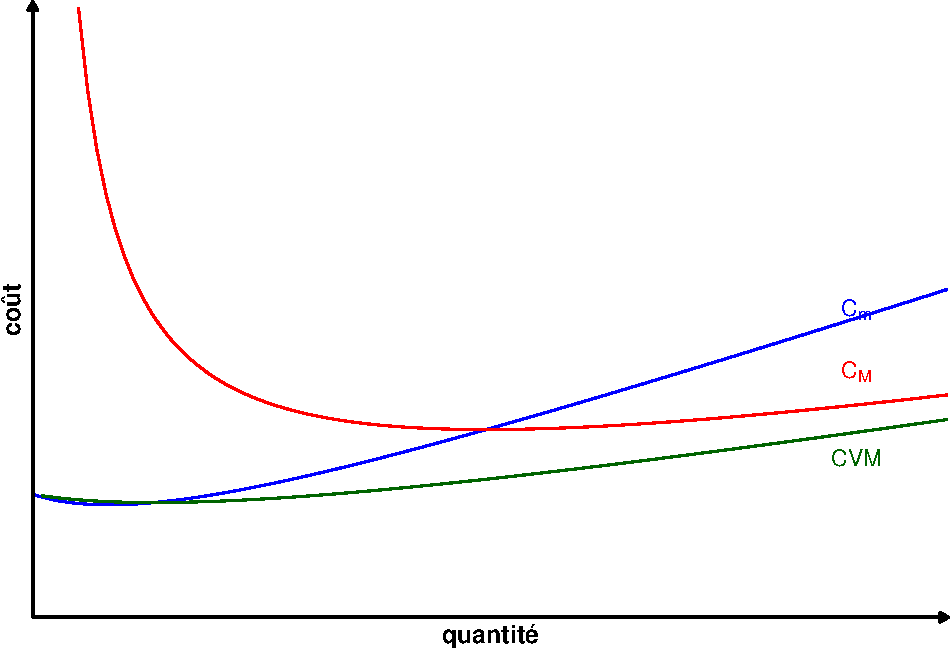
\includegraphics{_main_files/figure-latex/cppcout-1.pdf}
\caption{\label{fig:cppcout}Exemples de fonctions de coût.}
\end{figure}

\hypertarget{loffre-du-producteur}{%
\subsection{L'offre du producteur}\label{loffre-du-producteur}}

\begin{definition}[Recette totale]
La recette totale, notée \(RT\), est la recette issue de la vente des biens.
Pour \(q\) unités de bien vendus, le producteur gagne \(RT(q)\), autrement dit, c'est le chiffre d'affaire du producteur (pour ce bien).
\end{definition}

\begin{definition}[Recette marginale]
La recette marginale, notée \(R_m\) est la recette rapportée par une unité supplémentaire de bien vendue.
\[R_m(q)=RT'(q)\]
\end{definition}

\begin{definition}[Profit]
Le profit, noté \(\pi\) est la différence entre la recette totale et le coût total de production :
\[\pi(q)=RT(q)-CT(q)\]
\end{definition}

\begin{hypothesis}[Programme du producteur]
\protect\hypertarget{hyp:programmeproducteur}{}\label{hyp:programmeproducteur}Le producteur choisit la quantité produite de manière à maximiser son profit.
Mathématiquement, il résout le programme suivant :
\[\max_q\pi(q)=\max_q RT(q)-CT(q)\]
\end{hypothesis}

\begin{theorem}[Offre du producteur]
En concurrence pure et parfaite, le programme du producteur est tel que la quantité produite \(q\) égalise le coût marginal et la recette marginale :
\begin{equation}
R_m(q) =C_m(q)
\label{eq:cppopti}
\end{equation}
\end{theorem}

\begin{proof}
Le programme du producteur est de maximiser son profit :
\[\max_q\pi(q)=\max_q RT(q)-CT(q)\]
À l'optimum, et à condition que les fonctions de coût et de recette soient dérivables (ce qui sera toujours le cas dans ce cours). La condition du premier ordre s'écrit :
\[\pi'(q)=0\Leftrightarrow RT'(q)-CT'(q)=0\Leftrightarrow R_m(q)=C_m(q)\]
On obtient donc l'équation \eqref{eq:cppopti}.
\end{proof}

L'intuition pour ce résultat est la suivante.
Si la recette marginale est supérieure au coût marginal (\(R_m(q)>C_m(q)\)), alors augmenter la quantité produite rapporte plus que cela ne coûte et donc augmente le profit.
À l'inverse, si la recette marginale est inférieure au coût marginal (\(R_m(q)<C_m(q)\)), diminuer la quantité produite diminue plus le coût que la recette du producteur et donc augmente le profit.
La situation s'équilibre donc pour \(R_m(q)=C_m(q)\).
Si cette égalité n'est pas vérifiée, le producteur peut en effet augmenter son profit en jouant sur la quantité produite.

\begin{figure}
\centering
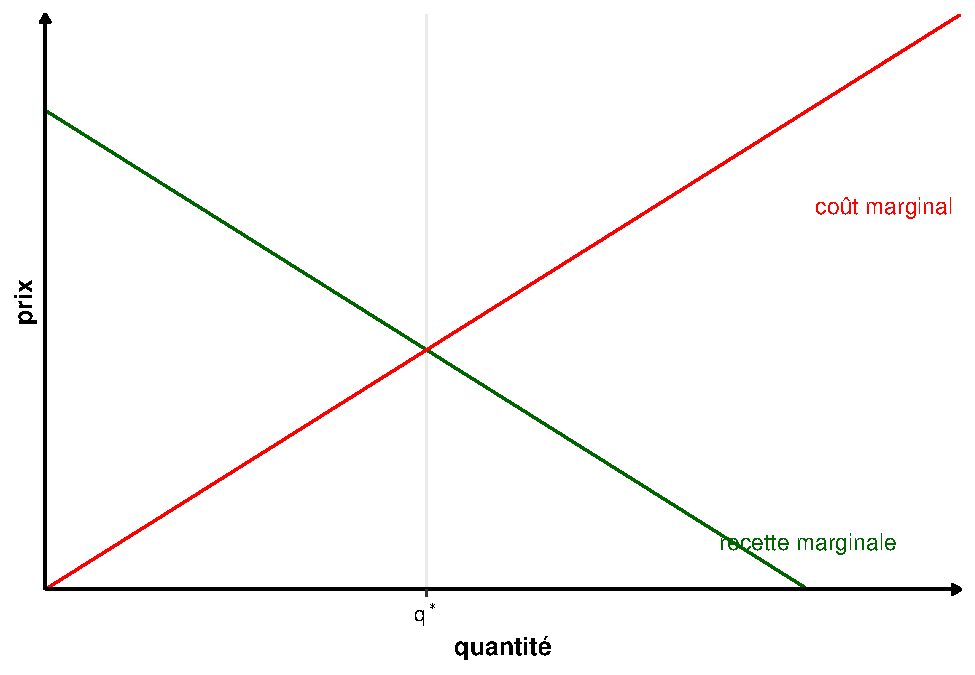
\includegraphics{_main_files/figure-latex/profixmax-1.pdf}
\caption{\label{fig:profixmax}Maximisation du profit du producteur.}
\end{figure}

En concurrence pure et parfaite, le producteur est \emph{price-taker}.
Le prix sur le marché est unique et donné , il vaut \(p\) et ne dépend pas des quantités produites par \emph{un} producteur.
Le producteur vend son bien au prix défini par le marché.
La recette totale devient donc \(RT(q)=p\times q\), avec \(p\) fixé.
La recette marginale est donc \(R_m(q)=RT'(q)=p\).
En réécrivant l'équation \eqref{eq:cppopti}, on obtient en concurrence pure et parfaite :
\[p=C_m(q)\]

\begin{proposition}[Courbe d'offre en CPP]
En concurrence pure et parfaite, la courbe d'offre du producteur est la courbe de coût marginal.
\[p=C_m(q)\]
\end{proposition}

Le profit du producteur s'écrit alors :
\[\pi(q)=RT(q)-CT(q)=pq-CT(q)=pq-C_M(q)q=q(p-C_M(q))\]
\begin{equation}
\pi(q)=q(p-C_M(q))
\label{eq:profitCM}
\end{equation}
L'équation \eqref{eq:profitCM} nous dit que le profit d'un producteur en concurrence pure et parfaite est la différence entre le prix de vente et le coût moyen de production multiplié par le nombre d'unités vendues.
Si ce prix est inférieur au coût moyen de toutes les unités vendues, le profit sera négatif.

\begin{figure}
\centering
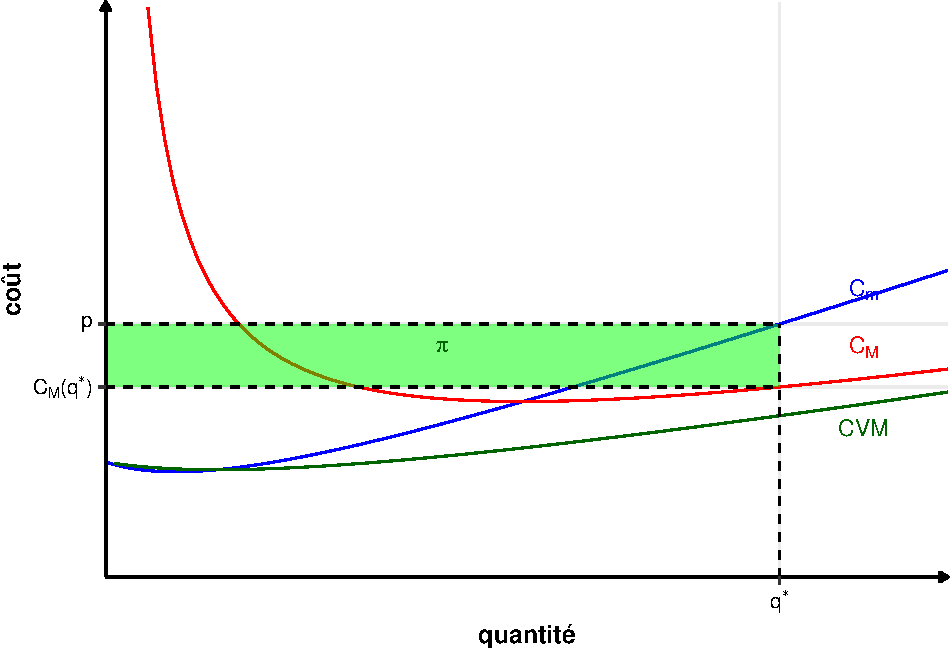
\includegraphics{_main_files/figure-latex/cppprofit-1.pdf}
\caption{\label{fig:cppprofit}Profit d'un producteur en concurrence pure et parfaite.}
\end{figure}

\hypertarget{luxe9quilibre-de-marchuxe9}{%
\section{L'équilibre de marché}\label{luxe9quilibre-de-marchuxe9}}

\begin{definition}[Demande agrégée (D)]
La \emph{demande agrégée (D)} est la somme des demandes individuelles pour chaque niveau de prix.
\end{definition}

La courbe de demande correspond à la suite des prix de réserve des individus, c'est-à-dire aux prix maximaux que chaque individu est prêt à payer pour obtenir une unité \emph{supplémentaire} du bien.

\begin{definition}[Offre agrégée (S)]
L'\emph{offre agrégée (S)} est la somme des offres individuelles pour chaque niveau de prix.
\end{definition}

La courbe d'offre correspond à la série des coûts marginaux de production, c'est-à-dire aux prix minimaux auxquels les producteurs souhaitent vendre une unité supplémentaire du bien.

\begin{definition}[Équilibre de marché]
L'équilibre de marché se fait à l'intersection entre l'offre agrégée (S) et la demande agrégée (D) (quand S=D).
\end{definition}

À l'équilibre de marché, on obtient une quantité d'équilibre (notée \(q^*\)) et un prix d'équilibre (noté \(p^*\)).
La vente de toutes les unités jusqu'à la quantité d'équilibre \(q^*\) au prix \(p^*\) procure un \emph{surplus} aux agents économiques.

\begin{figure}
\centering
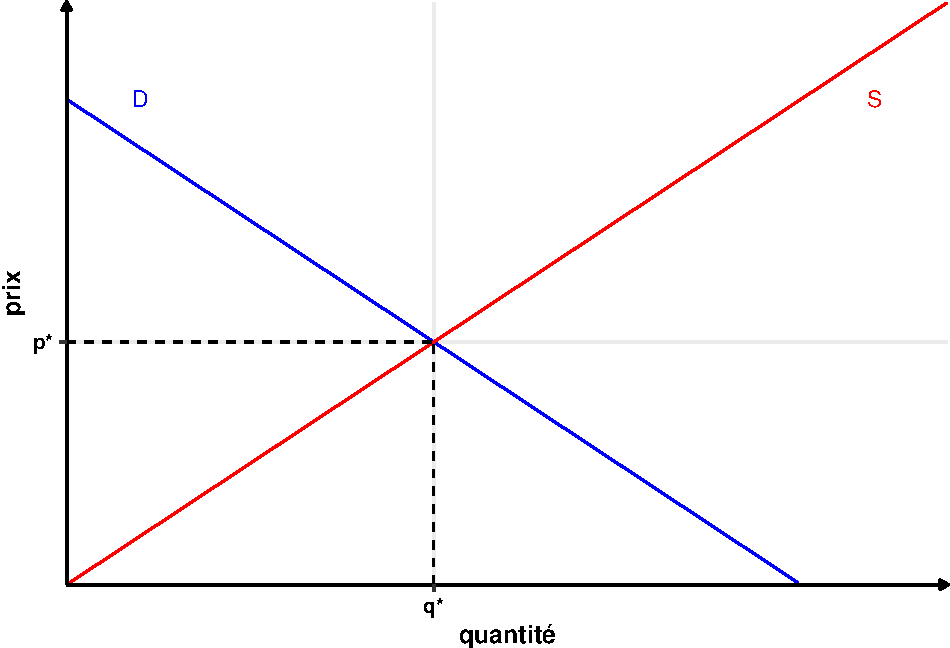
\includegraphics{_main_files/figure-latex/marche-1.pdf}
\caption{\label{fig:marche}Equilibre de marché.}
\end{figure}

\begin{definition}[Surplus des consommateurs]
Le surplus des consommateurs est la somme des différences entre le prix de réserve des consommateurs et le prix payé par le consommateur pour obtenir les biens.
Sur le graphique quantité prix \((q, p)\), c'est l'aire comprise entre la courbe de demande et la droite horizontale dont l'ordonnée est le prix d'échange.
Formellement :
\[S_c=\int_0^{q^*}P(q)-p^* dq\]
\end{definition}

\begin{remark}
Seule la dernière unité de bien achetée par les consommateur l'est au prix de réserve.
Il n'y a pas de gain à l'échange pour cette unité, mais pour toutes les autres, il y en a, ce qui explique pourquoi il y a un surplus à l'échange, et pourquoi celui-ci a lieu.
\end{remark}

\begin{definition}[Surplus des producteurs]
Le surplus des producteurs est la somme des différences entre le prix auquel les producteurs vendent le bien et la courbe de coût marginal, qui représente le coût d'une unité supplémentaire produite.
Sur le graphique quantité prix \((q, p)\), c'est l'aire comprise entre le prix de vente et la courbe de coût marginal.
Formellement :
\[S_p=\int_0^{q^*}p^*-S(q) dq\]
\end{definition}

En pratique, on utilisera jamais la formule avec des intégrales, mais on calculera l'aire du triangle (ou trapèze) concerné.

\begin{figure}
\centering
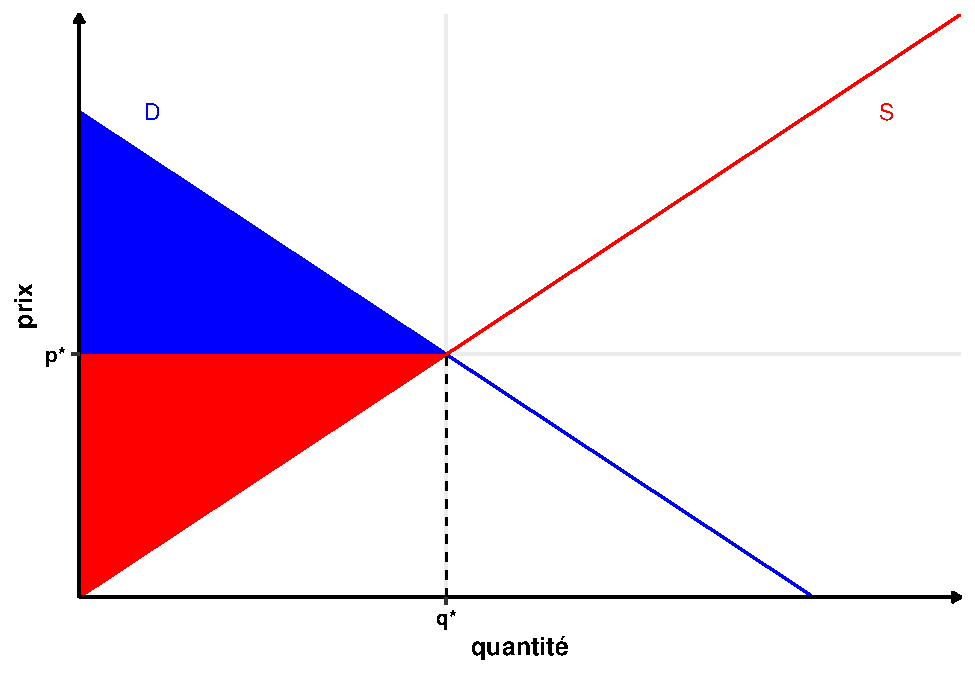
\includegraphics{_main_files/figure-latex/surplus-1.pdf}
\caption{\label{fig:surplus}Surplus des consommateurs et des producteurs.}
\end{figure}

\begin{proposition}[Propriétés de l'équilibre en concurrence pure et parfaite]
\protect\hypertarget{prp:cppprop}{}\label{prp:cppprop}L'équilibre en CPP \textbf{maximise} le \emph{surplus total}.
Tout autre couple prix/quantité abouti à un surplus total plus faible.\\
L'équilibre en CPP est \emph{Pareto-optimal}, i.e., il est impossible d'améliorer la situation d'un agent sans détériorer celle d'un autre.
C'est ce qu'on appelle le \emph{premier théorème du bien-être}.
\end{proposition}

Ces propriétés font de la CPP une ``référence'' par rapport à laquelle on peut comparer les résultats des autres structures de marché.

\hypertarget{perception-par-les-agents-isoluxe9s}{%
\section{Perception par les agents isolés}\label{perception-par-les-agents-isoluxe9s}}

L'hypothèse d'atomicité indique que les agents individuels sont isolés au sein d'un très grand nombre d'autres agents.
Ainsi, aucun agent n'a d'influence sur le prix s'il modifie son comportement.
Une conséquence directe est que le comportement des autres agents est perçu comme étant infiniment élastique.
C'est-à-dire qu'un producteur sait qu'au prix de marché, il pourra vendre toute sa production, mais que s'il pratique un prix même légèrement plus élevé, il ne vendra \textbf{rien}.
Il perçoit ainsi une demande infiniment élastique au prix, au niveau du prix \(p^*\).

\begin{figure}

{\centering 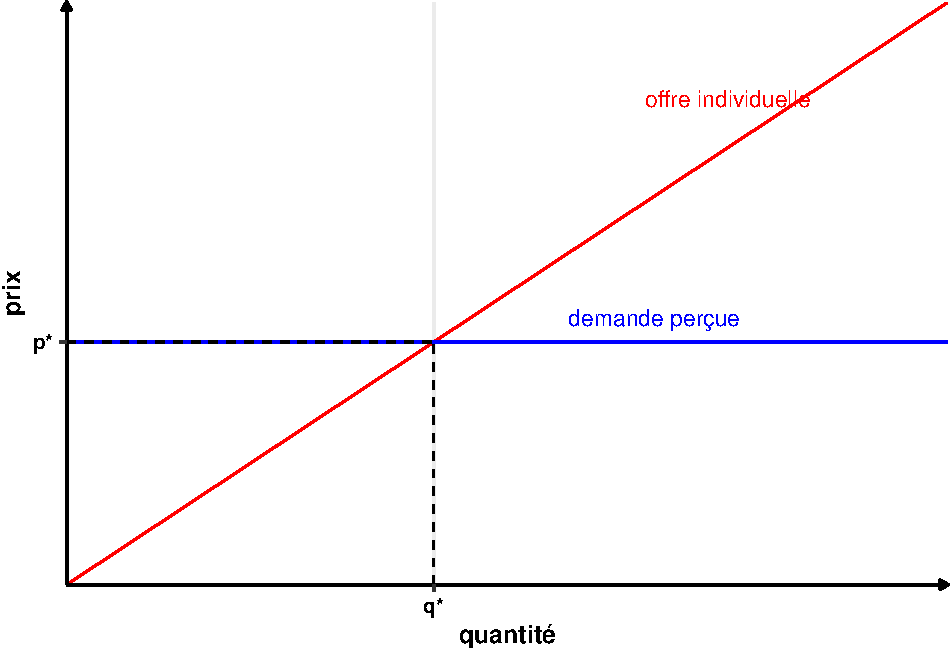
\includegraphics{_main_files/figure-latex/elasticite-1} 

}

\caption{Perception de la demande globale par un producteur isolé.}\label{fig:elasticite}
\end{figure}

Dans la figure \ref{fig:elasticite}, \(q^*\) représente la production optimale de ce producteur quand il est seul.

\hypertarget{le-monopole}{%
\chapter{Le monopole}\label{le-monopole}}

\begin{definition}[Monopole]
Un \emph{monopole} est sur un marché donné l'unique entreprise qui produit le bien.
\end{definition}

C'est le cas extrême opposé à la concurrence pure et parfaite, du côté du producteur.
Il est intéressant à étudier car il nous renseigne sur les principaux aspects du comportement des entreprises dans les cas intermédiaires.

Il y a de nombreuses raisons qui aboutissent à l'existence de monopoles.
Les principales sont :

\begin{itemize}
\tightlist
\item
  Légales, à cause de réglementation particulières.
  C'est ce qu'on appelle en général des professions réglementées, comme les avocats, les bureaux de tabac, les taxis\ldots{}
\item
  Légales, à cause des brevets sur une technologie données (industrie pharmaceutique, \ldots) ;
\item
  Historique, le premier arrivé ;
\item
  Monopoles \emph{naturels} : en présence d'économies d'échelles, produire une quantité donnée revient moins cher avec un seul producteur qu'avec plusieurs.
  C'est notamment les cas des industries où il faut installer des réseaux (chemins de fer, électricité, téléphone, \ldots).
  Plus généralement, les industries avec des coûts fixes / coûts d'entrées très élevées aboutissent à des formes proches du monopole naturel (sidérurgie, automobile, \ldots) ;
\item
  Exclusivité sur la production de certaines matières premières (cuivre au Chili, terres rares en Chine, \ldots) ;
\item
  Coalitions créant un cartel ;
\item
  \ldots{}
\end{itemize}

\hypertarget{recette-et-recette-marginale}{%
\section{Recette et recette marginale}\label{recette-et-recette-marginale}}

\hypertarget{duxe9finition}{%
\subsection{Définition}\label{duxe9finition}}

À la différence du cas de la concurrence pure et parfaite, le monopole perçoit la courbe de demande agrégée, et non plus celle avec une élasticité infinie.
Le choix de la quantité qu'il met sur le marché modifie le prix auquel il pourra vendre sa production, et il le sait.
Il va choisir \textbf{un} des paramètres du couple \((q, P(q))\), et l'autre en découlera, à travers la demande inverse \(P(q)\).
Autrement dit, s'il choisit \(q\), \(P(q)\) sera déterminé par la demande (inverse).
Si, au contraire, il choisit \(P\), \(q\) sera déterminé par la demande.

En CPP, la recette totale du producteur individuel était \(R(q) = q\cdot P(q^*)\), où \(q\) est sa production individuel, \(q^*\) la quantité d'équilibre sur le marché (résultat de la production de \emph{toutes} les entreprises présentes sur le marché) et \(P(q^*)=p^*\) est le prix d'équilibre.

En monopole, le prix dépend de la production du monopole (ou l'inverse, peu importe) :
\[
R(q) = q\cdot P(q)
\]

\hypertarget{recette-marginale-et-courbe-de-demande}{%
\subsection{Recette marginale et courbe de demande}\label{recette-marginale-et-courbe-de-demande}}

Comme la courbe de demande est décroissante (l'élasticité prix de la demande est négative \(\varepsilon_{q/p} <0\)), \(P(q)\) et \(q\) ont une relation inverse.
Autrement dit, si \(q\) augmente, alors \(p\) baisse, et réciproquement.

Cela implique que la recette totale augmentera ou baissera suivant les propriétés de la courbe de demande.

\begin{figure}
\centering
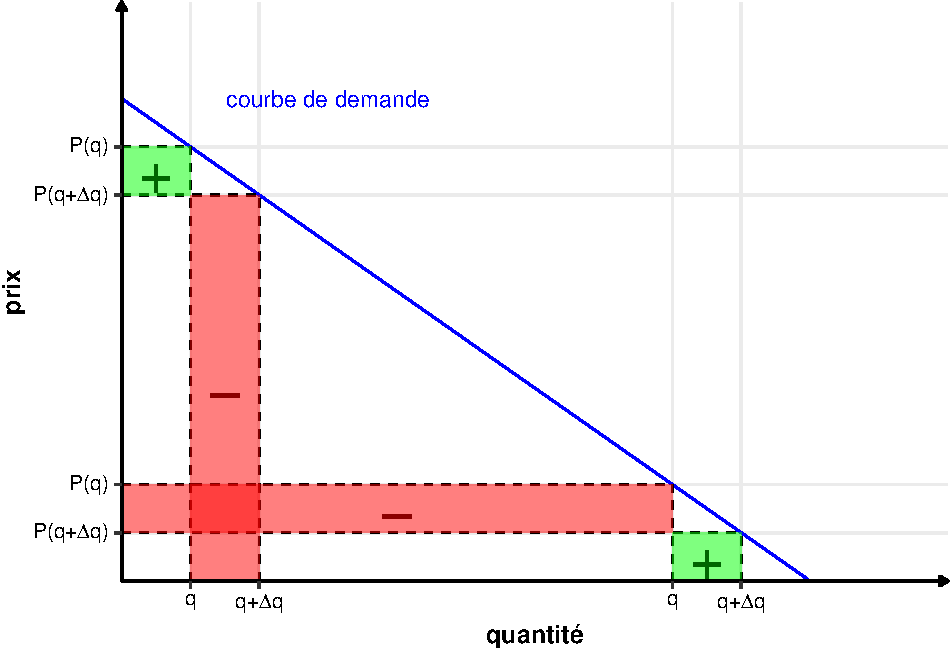
\includegraphics{_main_files/figure-latex/monorecettemarginale-1.pdf}
\caption{\label{fig:monorecettemarginale}Recette marginale d'un monopole.}
\end{figure}

Quel est le paramètre important de la courbe de demande qui détermine si le revenu \(R\) augmente ou diminue (c'est-à-dire si \(R_m\) est positive ou négative) ?

\begin{align*}
R(q) & = qP(q)\\
R_m(q)& = R'(q) \\
& = \left(qP(q)\right)' \\
& = P(q) + qP'(q) \\
& = P(q)\left(1 + \frac{q}{P(q)}P'(q) \right)\\
& = P(q)\left(1 + \frac{1}{\varepsilon_{q/p}(q)}\right)
\end{align*}

\begin{remark}[Élasticité prix de la demande]
L'élasticité prix de la demande \(\varepsilon_{q/p}\) s'écrit :
\[\varepsilon_{q/p}(p)=\frac{p}{D(p)}D'(p) <0\]
Où \(D\) est la fonction de demande.
Elle est toujours négative, car la demande diminue quand le prix augmente.
On peut la réécrire à l'aide de la fonction de demande inverse \(P\).
Comme \(D\) et \(P\) sont les fonctions réciproques l'une de l'autre, on a \(D(P(q)) = q\).
En dérivant à gauche et à droite, on obtient :
\[P'(q)D'(P(q)) = 1\]
On obtient donc :
\[P'(q)=\frac{1}{D'(p)}\]
Et l'élasticité prix de la demande peut aussi s'écrire :
\[\varepsilon_{q/p}(q)=\frac{P(q)}{q}\frac{1}{P'(q)}\]
\end{remark}

On peut donc écrire :
\begin{equation}
R_m(q) = P(q)\left(1 - \frac{1}{|\varepsilon_{q/p}(q)|}\right)
\label{eq:rm}
\end{equation}

De l'équation \eqref{eq:rm}, on observe que le signe de la recette marginale \(R_m\) dépend de l'élasticité prix de la demande.

\begin{enumerate}
\def\labelenumi{\arabic{enumi}.}
\tightlist
\item
  Si la demande est élastique (\(|\varepsilon_{q/p}(q)|>1\)), alors \(R_m(q)>0\), donc si la quantité augmente, le revenu augmente.
\item
  Si la demande est inélastique (\(|\varepsilon_{q/p}(q)|<1\)), alors \(R_m(q)<0\), donc si la quantité augmente, le revenu diminue.
\end{enumerate}

Une représentation graphique de l'allure générale est donnée dans la figure \ref{fig:monopoleelasticite}

\begin{figure}
\centering
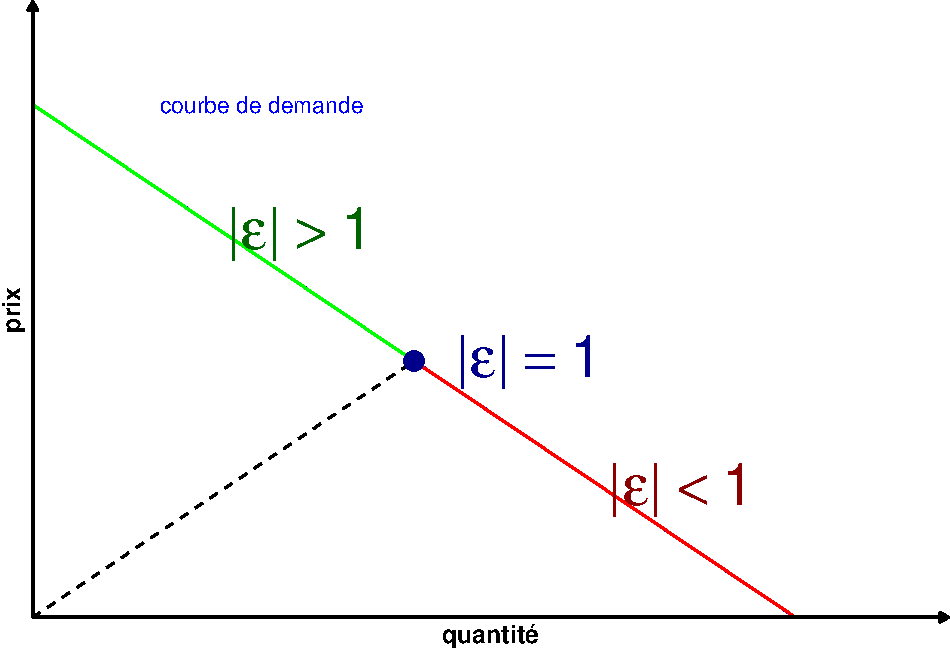
\includegraphics{_main_files/figure-latex/monopoleelasticite-1.pdf}
\caption{\label{fig:monopoleelasticite}La recette marginale est maximale lorsque l'élasticité prix de la demande est égale à -1.}
\end{figure}

\hypertarget{repruxe9sentation-graphique}{%
\subsection{Représentation graphique}\label{repruxe9sentation-graphique}}

La courbe de recette marginale est toujours située en-dessous de la courbe de demande :
\[
R_m(q) = P(q) + qP'(q) < P(q)
\]
et \(P'(q)\) est négative (la demande inverse est décroissante).

\hypertarget{exemple-avec-une-courbe-de-demande-linuxe9aire}{%
\subsubsection{Exemple avec une courbe de demande linéaire}\label{exemple-avec-une-courbe-de-demande-linuxe9aire}}

Prenons maintenant l'exemple d'une courbe de demande inverse linéaire quelconque \(P(q) = a-bq\) (\(a\) et \(b\) sont des paramètres quelconques).
On obtient alors \(R_m(q) = a-2bq\) (et \(R(q) = aq-bq^2\)).\\
Dans le cas linéaire, le revenu marginal est une droite de pente deux fois plus élevée que la demande, et ayant la même ordonnée à l'origine.
La recette marginale divise en deux tout segment horizontal entre l'axe des ordonnées et la courbe de demande inverse.
On peut ainsi représenter graphiquement, comme dans la figure \ref{fig:recettemarginale} la demande, la recette marginale et la recette totale.

\begin{figure}
\centering
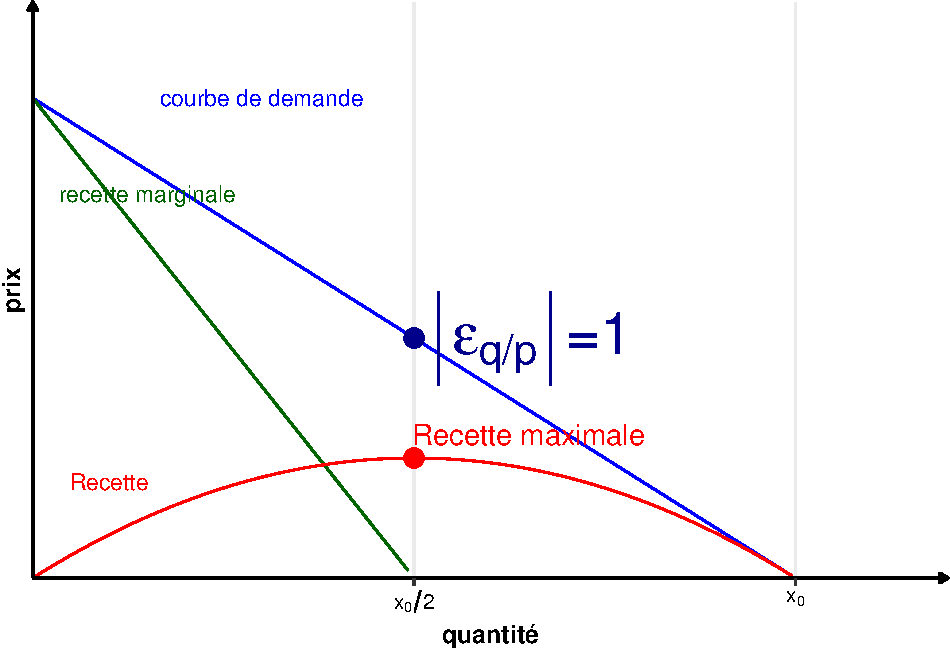
\includegraphics{_main_files/figure-latex/recettemarginale-1.pdf}
\caption{\label{fig:recettemarginale}Elasticité et recette.}
\end{figure}

La recette maximale est atteinte lorsque la valeur absolue de l'élasticité prix de la demande est égale à 1 (\(|\varepsilon_{q/p}(q)|=1\)).

\begin{figure}
\centering
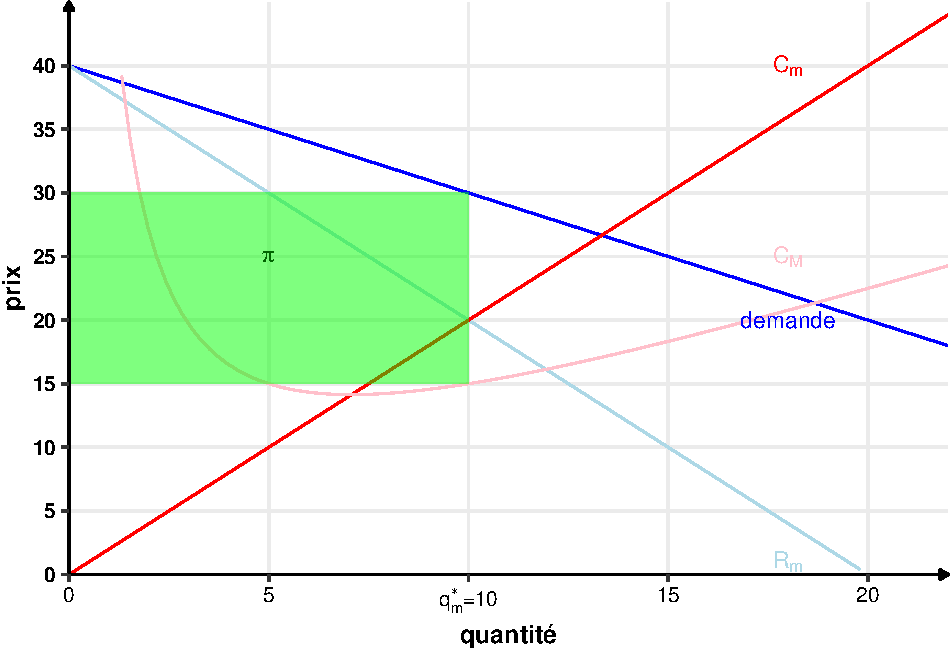
\includegraphics{_main_files/figure-latex/monopoleprofit-1.pdf}
\caption{\label{fig:monopoleprofit}Recette maximale.}
\end{figure}

Sur la figure \ref{fig:monopoleprofit}, on voit qu'il est possible de calculer la recette totale de deux manières :

\begin{enumerate}
\def\labelenumi{\arabic{enumi}.}
\tightlist
\item
  En utilisant l'aire du trapèze vert (intégrale de la recette marginale entre 0 et la quantité échangée \(q^*\)) ;
\item
  En utilisant l'aire du rectangle rouge (\(\pi=p^* q^*\)).
\end{enumerate}

Le résultat donne l'égalité d'aire entre le triangle vert et le triangle rouge.

\hypertarget{duxe9cision-de-production-du-monopole}{%
\section{Décision de production du monopole}\label{duxe9cision-de-production-du-monopole}}

\hypertarget{maximisation-du-profit}{%
\subsection{Maximisation du profit}\label{maximisation-du-profit}}

Comme dans le cas de la CPP, on suppose que le monopole cherche à maximiser son profit \(\pi(q)=R(q)-C(q)\), où \(C(q)\) est la fonction de coût (total) du monopole.\\
Il y a 2 conditions d'optimalités, les conditions de premier ordre (la dérivée du profit à l'optimum est nulle: \(\pi'(q^*)=0\)) et de second ordre (la dérivée seconde du profit à l'optimum est strictement négative \(\pi''(q^*)<0\)), ainsi qu'une contrainte, que le profit à l'optimum soit positif (\(\pi(q^*)>0\)).

La condition de premier ordre s'exprime ainsi :
\[
\begin{array}{rcl}
\pi'(q^*) &=&0\\
\Leftrightarrow R'(q^*) - C'(q^*) &=& 0\\
\Leftrightarrow R_m(q^*) &=&C_m(q^*) 
\end{array}
\]
À l'optimum, le monopole égalise le coût marginal et le revenu marginal.

La condition du second ordre s'exprime ainsi :
\[
\begin{array}{rcl}
\pi''(q^*) &<&0\\
\Leftrightarrow R_m'(q^*) - C_m'(q^*) &<& 0\\
\Leftrightarrow R_m'(q^*) &<& C_m'(q^*)
\end{array}
\]

La dérivée de la recette marginale doit être inférieure à la dérivée du coût marginal.
Autrement dit, la recette marginale doit croître moins vite que le coût marginal.
Cette condition est en particulier vérifiée si la recette marginale est décroissante et le coût marginal croissant.

Finalement, il faut vérifier que le profit à l'optimum est positif (\(\pi(q^*)>0\)).
Dans le cas contraire, le marché n'existerait tout simplement pas, car le monopole ne voudrait pas produire le bien.

\begin{theorem}[Optimum du du monopole]
À l'optimum, le monopole égalise le coût marginal et le revenu marginal.
Ce n'est un maximum que si la dérivée de la recette marginale est inférieure à la dérivée du coût marginal et que le profit est positif.
\begin{equation}
R_m(q^*)=C_m(q^*) 
\label{eq:cpo}
\end{equation}
\begin{equation}
R_m'(q^*) <C_m'(q^*) \label{eq:cso}
\end{equation}
\begin{equation}
\pi(q^*)>0 \label{eq:profitpos}
\end{equation}
\end{theorem}

On peut comprendre graphiquement pourquoi il faut que le coût marginal et la recette marginale soient égaux (figure \ref{fig:monopoleoptimale}).
Si le monopole produit plus que \(q_m^*\), alors chaque unité produite en plus lui coûte plus chère qu'elle ne lui rapporte.
A l'inverse, s'il produit moins, produire des unités en plus lui rapporterait plus que cela ne lui coûte.

\begin{figure}
\centering
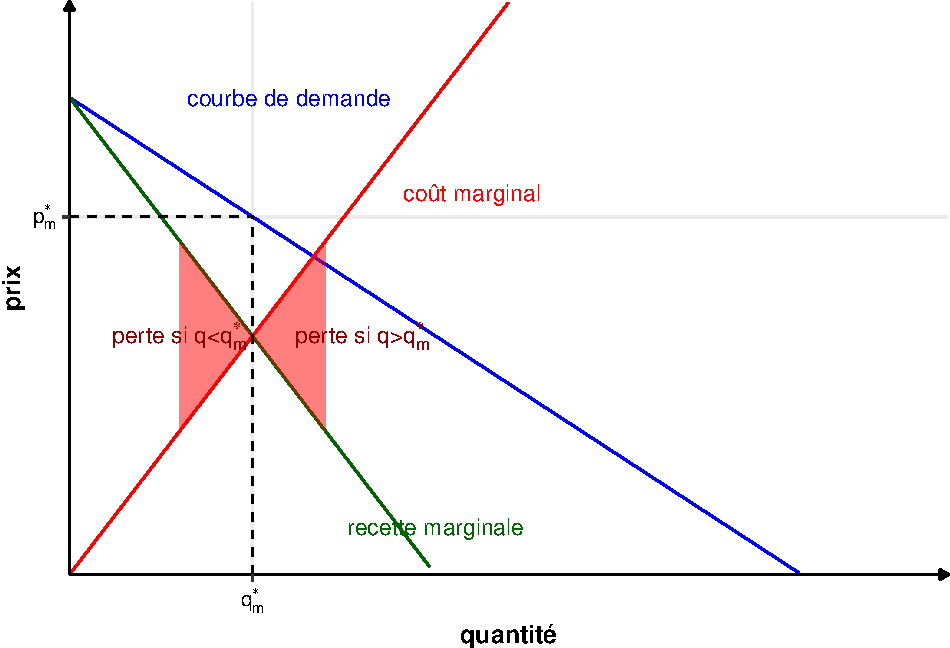
\includegraphics{_main_files/figure-latex/monopoleoptimale-1.pdf}
\caption{\label{fig:monopoleoptimale}Production optimale du monopole.}
\end{figure}

Le prix est lu et obtenu sur la courbe de \textbf{demande}.

\begin{example}[Maximisation du monopole]
\protect\hypertarget{exm:monopoleexemple}{}\label{exm:monopoleexemple}Prenons un monopole avec une fonction de coût \(C(q)=50+q^2\).
Le monopole fait face à une demande inverse \(P(q) = 40-q\).

Le coût marginal est :
\[
C_m(q) = C'(q)=2q
\]

La recette totale est :
\[
R(q) = qP(q) = q(40-q) = 40q-q^2
\]
La recette marginale est donc :
\[
R_m(q) = R'(q) = 40 - 2q
\]
Le profit vaut :
\[
\pi(q) = R(q)-C(q)
\]
Conformément à l'équation \eqref{eq:cpo}, il est maximal lorsque :
\[
\begin{array}{rcl}
R_m(q^*) &=&C_m(q^*)\\
\Leftrightarrow 40 -2q &= &2q\\
\Leftrightarrow q^*&=&10
\end{array}
\]
La condition de second ordre de l'équation \eqref{eq:cso} est bien vérifiée, car \(-2<2\).

Le prix de vente vaut :
\[P(q^*) = P(10) = 40-10 = 30\]
La recette vaut 300, le coût 150.
On a donc un profit de \textbf{150}, qui est bien positif (condition de l'équation \eqref{eq:profitpos}.
\end{example}

\begin{figure}
\centering
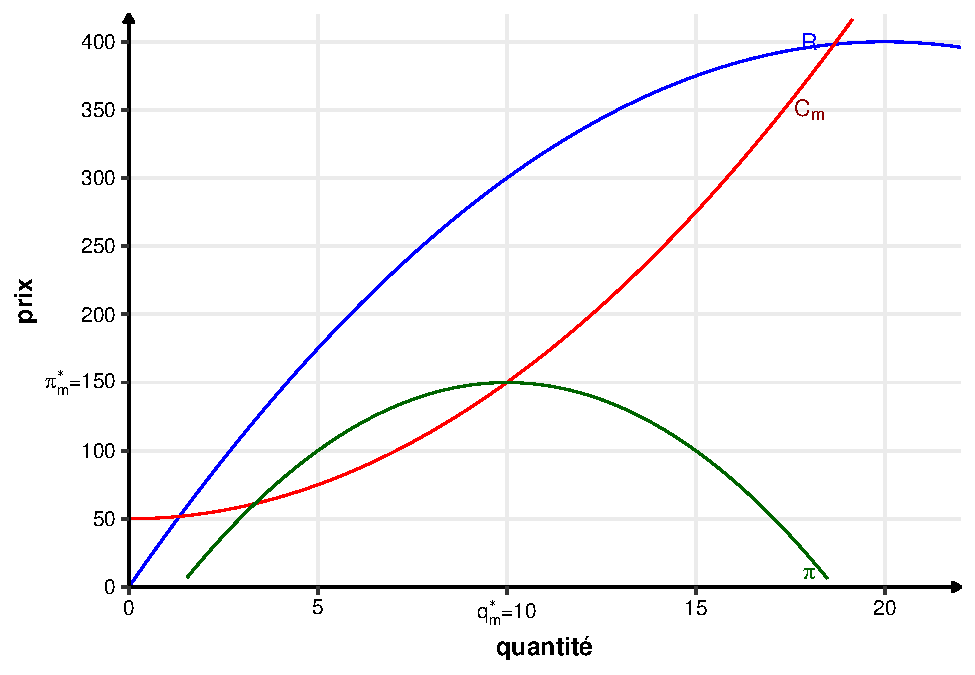
\includegraphics{_main_files/figure-latex/monopolerecette-1.pdf}
\caption{\label{fig:monopolerecette}Recette, coût et profit dans l'exemple \ref{exm:monopoleexemple}.}
\end{figure}

\begin{figure}
\centering
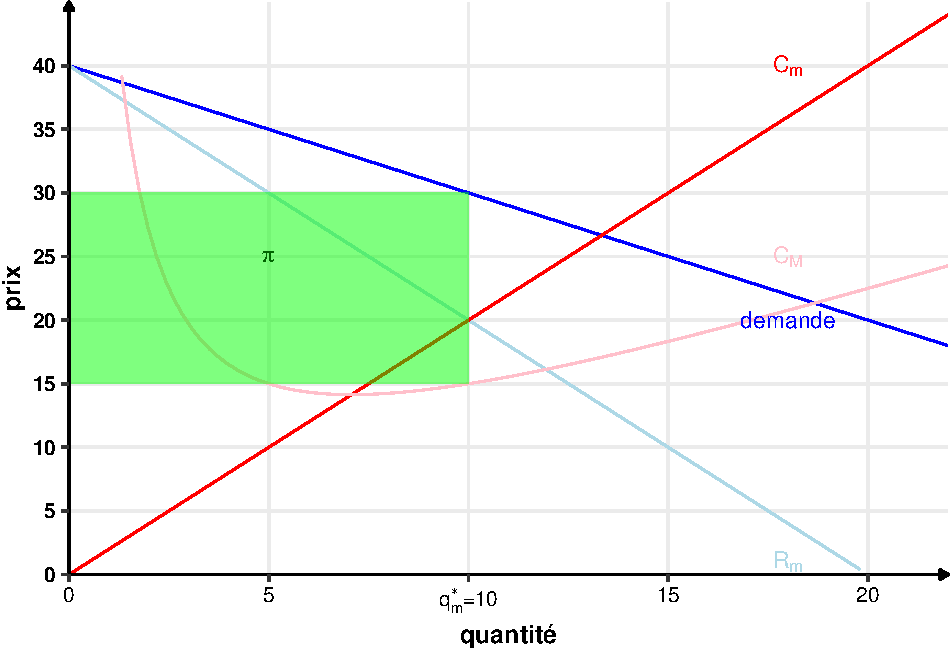
\includegraphics{_main_files/figure-latex/monopoleprofitexemple-1.pdf}
\caption{\label{fig:monopoleprofitexemple}Demande, prix, coûts et profits dans l'exemple \ref{exm:monopoleexemple}.}
\end{figure}

\hypertarget{propriuxe9tuxe9s-de-la-solution-du-monopole}{%
\subsection{Propriétés de la solution du monopole}\label{propriuxe9tuxe9s-de-la-solution-du-monopole}}

On avait dans l'équation \eqref{eq:rm} :
\[
R_m(q) = P(q)\left(1 - \frac{1}{|\varepsilon_{q/p}(q)|}\right)
\]
Comme à l'optimum, d'après l'équation \eqref{eq:cpo}, on doit avoir \(R_m(q^*)=C_m(q^*)\), on a :
\[
R_m(q^*) = P(q^*)\left(1 - \frac{1}{|\varepsilon_{q/p}(q^*)|}\right) = C_m(q^*) 
\label{eq:rmcm}
\]
On observe ici un lien avec la solution en CPP.
En effet, en CPP, l'élasticité de la demande au prix est perçue comme infinie, on aura donc bien \(P(q^*) = C_m(q^*)\), la solution obtenue en CPP.
Dès lors que l'élasticité de la demande au prix n'est plus infinie en revanche, on obtient :
\[
 P(q^*)=\frac{C_m(q^*)}{1 - \frac{1}{\left|\varepsilon_{q/p}(q^*)\right|}} > C_m(q^*)
\]

\emph{Question :} Dans quelle zone d'élasticité le monopole opère-t-il ?

Si \(\left|\varepsilon_{q/p}(q^*)\right|<1\), c'est-à-dire que si la demande est inélastique, alors \(1 - \frac{1}{\left|\varepsilon_{q/p}(q^*)\right|} <0\), ce qui implique que la recette marginale \(R_m\) est négative, et donc impossible à égaliser avec le coût marginal \(C_m\).\\
On peut voir la réponse d'une autre façon.
Si la pente est inélastique, alors le revenu \(R\) augmente quand la quantité \(q\) baisse.
Le coût total \(C\) baisse aussi quand la quantité baisse.
Le monopole aurait donc tout intérêt à réduire sa production lorsque la demande est inélastique.

\begin{corollary}
Le monopole opère donc nécessairement dans la zone élastique de la courbe de demande : \(\left|\varepsilon_{q/p}(q^*)\right|>1\) .
\end{corollary}

\hypertarget{indice-de-pouvoir-du-monopole}{%
\subsection{Indice de pouvoir du monopole}\label{indice-de-pouvoir-du-monopole}}

La capacité du monopole à vendre à un prix supérieur au coût marginal dépend de la plus ou moins grande élasticité de la demande au prix.
Cela permet de construire un indice du \emph{pouvoir de monopole} à partir de l'élasticité du prix à la demande à l'équilibre.
On a, d'après l'équation \eqref{eq:rmcm} :
\[
R_m(q^*) = P(q^*)\left(1 - \frac{1}{|\varepsilon_{q/p}(q^*)|}\right) = C_m(q^*) 
\]
On en déduit :

\[\begin{array}{rl}
& C_m(q^*) = P(q^*) - \frac{P(q^*)}{|\varepsilon_{q/p}(q^*)|}\\
\Leftrightarrow & P(q^*) - C_m(q^*) = \frac{P(q^*)}{|\varepsilon_{q/p}(q^*)|}
\end{array}
\]

\begin{definition}[Indice de Lerner]
\protect\hypertarget{def:Lerner}{}\label{def:Lerner}On définit l'indice de Lerner \(L\) par :
\[
L=\frac{1}{|\varepsilon_{q/p}(q^*)|} = \frac{P(q^*) - C_m(q^*)}{P(q^*)} \label{eq:Lerner}
\]
L'indice de Lerner est donc inversement proportionnel à l'élasticité prix de la demande.
Il est aussi égal à la capacité du monopole à vendre au-dessus de son coût marginal, en pourcentage du prix total.
\end{definition}

On peut construire à partir de l'équation précédente le \emph{markup pricing}.

\begin{definition}[Markup pricing]
\[
P(q^*) =\frac{|\varepsilon_{q/p}(q^*)|}{|\varepsilon_{q/p}(q^*)|-1} C_m(q^*)
\]
\end{definition}

\hypertarget{variation-de-la-demande}{%
\subsection{Variation de la demande}\label{variation-de-la-demande}}

Les décisions de production du monopole et la fixation de son prix dépendent de la demande à laquelle il fait face et du coût marginal.
Le monopole n'a \textbf{pas de courbe d'offre} au sens où il n'y a pas de relation univoque entre prix et quantité produite, à la différence des producteurs en CPP.
En monopole, si la demande change, le monopole s'adapte, soit en changeant sa production, mais pas son prix (figure \ref{fig:monopolechangementdemande2}), ou l'inverse (figure\ref{fig:monopolechangementdemande1}).

\begin{figure}
\centering
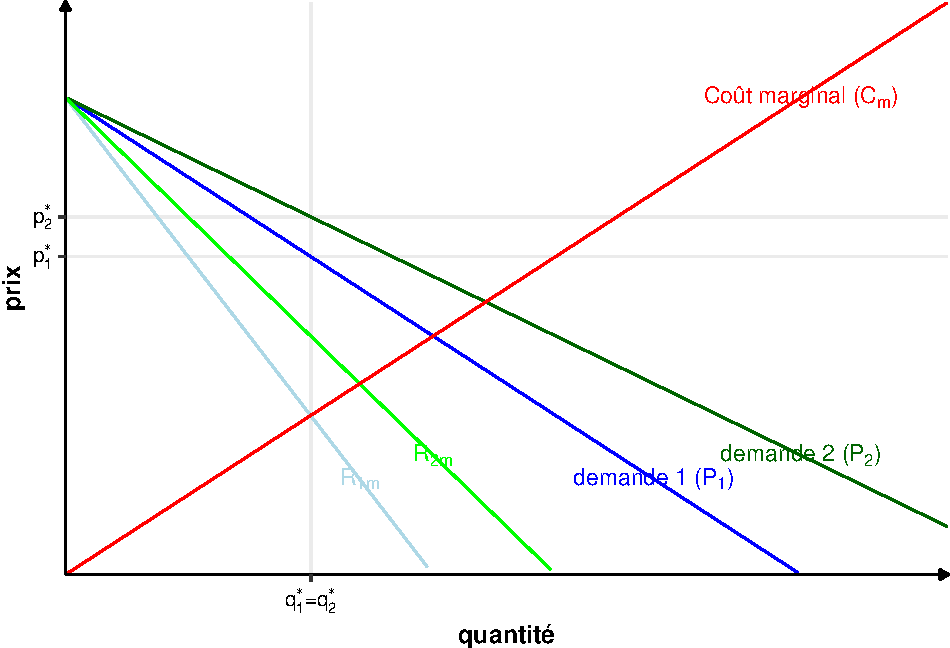
\includegraphics{_main_files/figure-latex/monopolechangementdemande1-1.pdf}
\caption{\label{fig:monopolechangementdemande1}Exemple de réaction du monopole à un changement de demande: changement de prix.}
\end{figure}

\begin{figure}
\centering
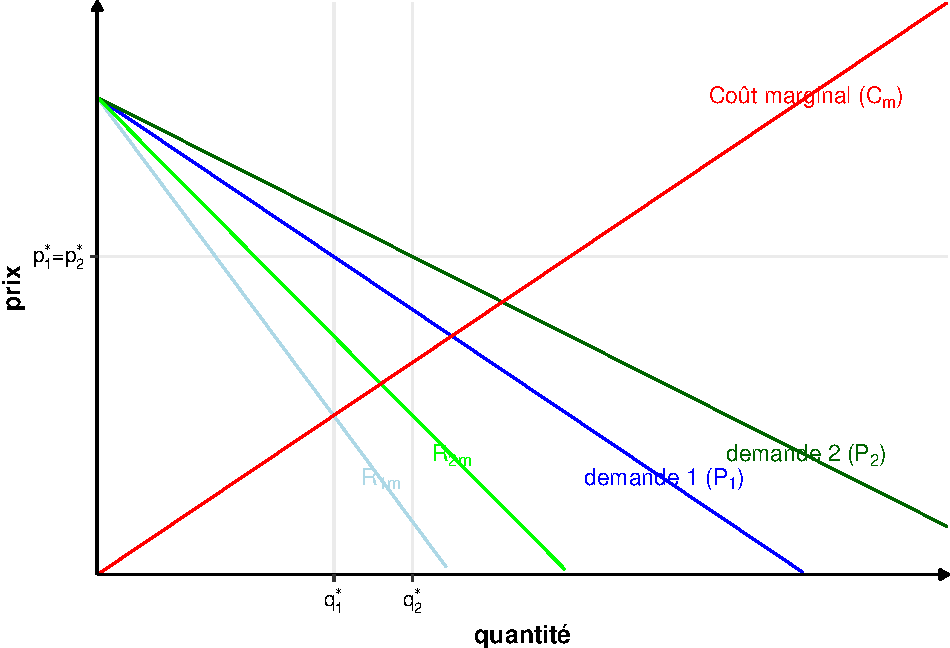
\includegraphics{_main_files/figure-latex/monopolechangementdemande2-1.pdf}
\caption{\label{fig:monopolechangementdemande2}Exemple de réaction du monopole à un changement de demande: changement de quantité.}
\end{figure}

En CPP, un changement de demande, si elle implique une changement du prix d'équilibre, entraîne forcément un changement dans la quantité produite par un producteur individuel.

\hypertarget{linefficience-du-monopole}{%
\subsection{L'inefficience du monopole}\label{linefficience-du-monopole}}

La production du monopole est inférieure à la production en CPP et le prix est supérieur au prix de CPP.

\begin{figure}
\centering
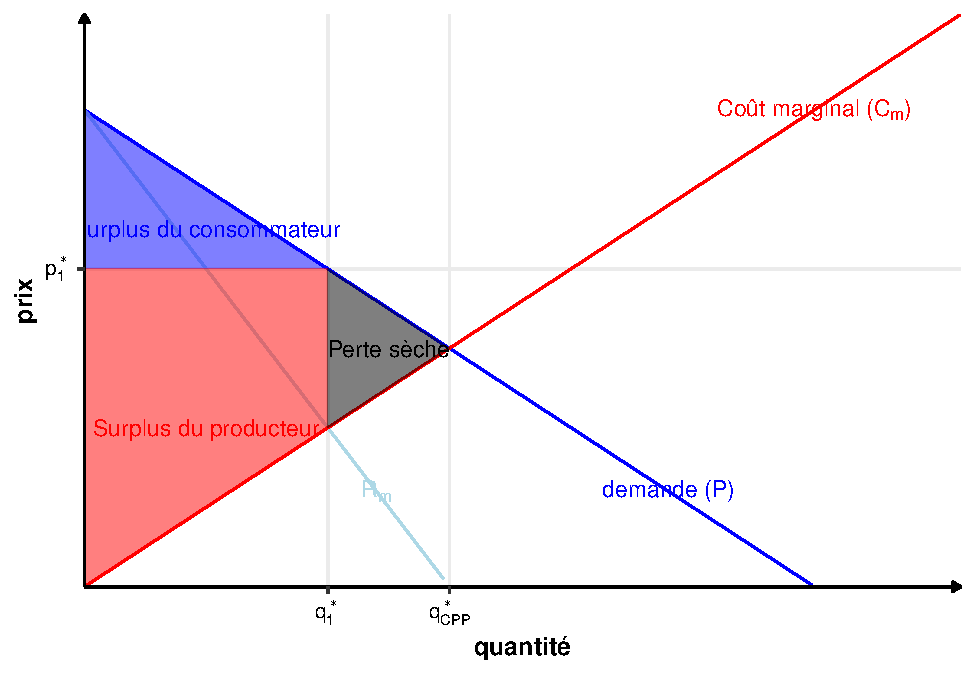
\includegraphics{_main_files/figure-latex/monosurplus-1.pdf}
\caption{\label{fig:monosurplus}Surplus quand le producteur est en monopole.}
\end{figure}

Cela implique que le surplus du producteur (son profit) est plus élevé en monopole qu'en CPP, et que le surplus des consommateur est plus faible.
Il y a globalement une perte sèche de surplus total.
\textbf{Le monopole est inefficace au sens de Pareto.}
Il existe des consommateurs prêt à acheter à un prix supérieur au coût marginal (dans le triangle de la perte sèche).
Il est donc possible d'avoir une amélioration parétienne qui améliore à la fois la situation des consommateurs et du monopole.
Il suffirait pour cela que le monopole produise une unité supplémentaire du bien à un prix supérieur au coût marginal, sans rien changer d'autre pour obtenir cette amélioration.

\hypertarget{ruxe9gulation-du-monopole}{%
\section{Régulation du monopole}\label{ruxe9gulation-du-monopole}}

Cette partie va traiter de la manière dont un gouvernement peut inciter ou contraindre un monopole à modifier son comportement.

\hypertarget{taxe-unitaire}{%
\subsection{Taxe unitaire}\label{taxe-unitaire}}

Un gouvernement impose une taxe de \(t\) unités monétaire par unité de bien produite.
On a donc :

\[
\pi(q) = R(q) - C(q) -tq
\]
La condition de première ordre de la maximisation du producteur de l'équation \eqref{eq:cpo} devient alors :
\[
\begin{array}{rl}
&(R(q)-C(q) -tq)'(q^*) = 0\\
\Leftrightarrow & R_m(q^*)-C_m(q*) -t = 0\\
\Leftrightarrow & R_m(q^*) = C_m(q^*) + t
\end{array}
\]
Le problème est exactement le même que précédemment, en intégrant la taxe dans le coût marginal.
Pour le monopole, c'est comme si l'État ajoutait un coût \(t\) à chaque unité produite, ce qui est effectivement ce que l'État fait.

\begin{figure}
\centering
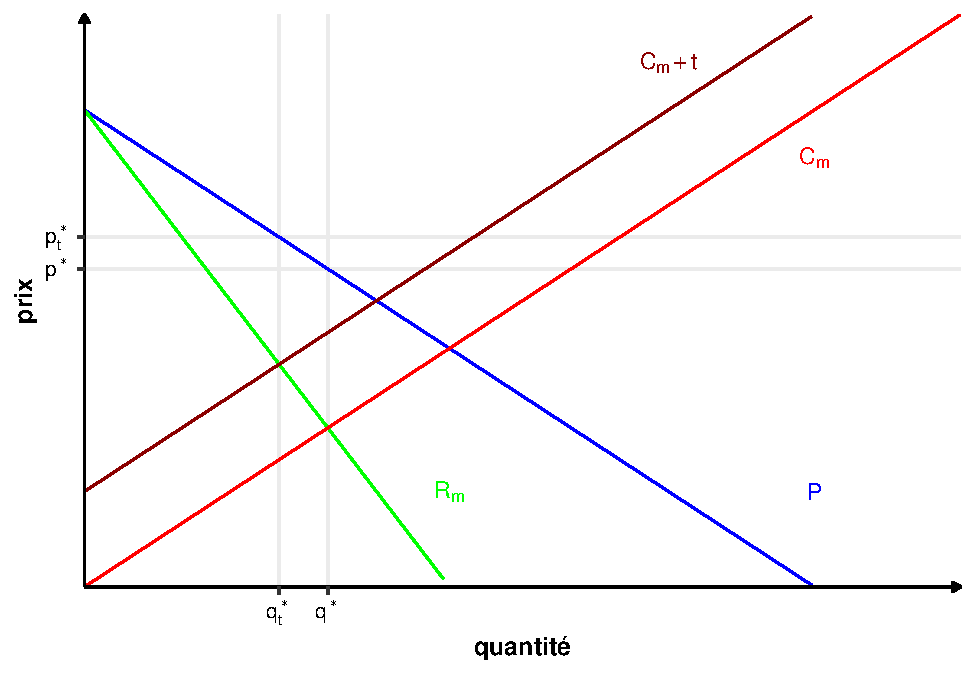
\includegraphics{_main_files/figure-latex/monopoletaxeunitaire-1.pdf}
\caption{\label{fig:monopoletaxeunitaire}Impact d'une taxe unitaire : augmentation du coût marginal.}
\end{figure}

Cela entraîne une diminution de la quantité produite et une augmentation du prix.
Le surplus des consommateurs baisse, ainsi que celui du monopole.

Une vue \textbf{alternative} à l'augmentation du coût marginal est de considérer que la taxe diminue la recette marginale de \(t\) :
\[
 R_m(q^*) -t = C_m(q^*)
\]

\begin{figure}
\centering
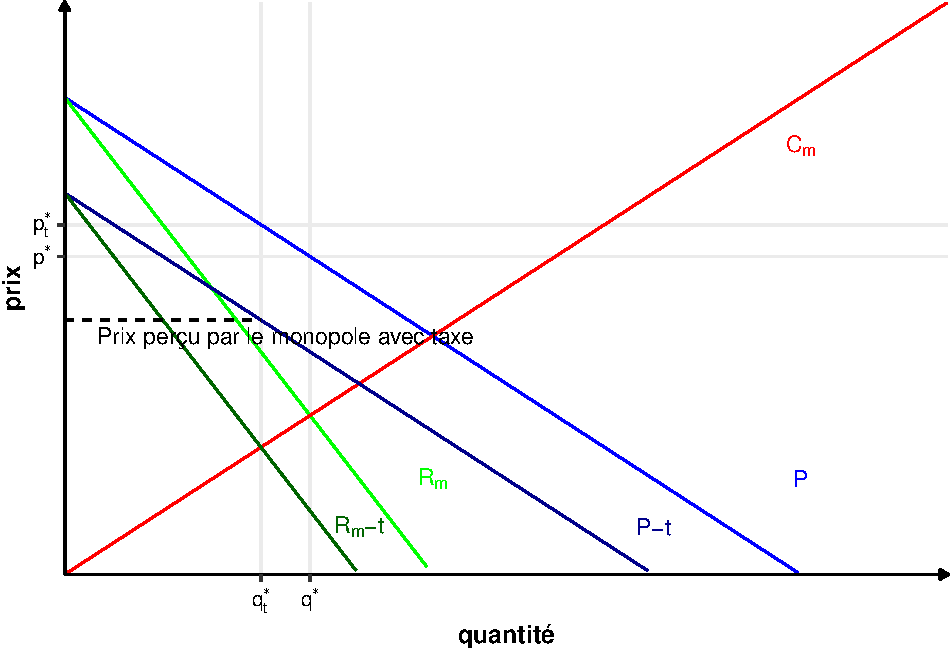
\includegraphics{_main_files/figure-latex/monopoletaxeunitaire2-1.pdf}
\caption{\label{fig:monopoletaxeunitaire2}Impact d'une taxe unitaire : diminution de recette marginale.}
\end{figure}

Si le gouvernement utilise une taxe négative (= une subvention), alors le gouvernement peut augmenter la production et de diminuer le prix.

\hypertarget{taxe-forfaitaire}{%
\subsection{Taxe forfaitaire}\label{taxe-forfaitaire}}

Avec une taxe forfaitaire, l'état prélève un montant \(T\) indépendant de la quantité produite sur le profit du producteur.
\[
\pi(q) = R(q) - C(q) -T
\]
La condition du premier ordre de l'équation \eqref{eq:cpo} devient alors :
\[
\begin{array}{rl}
& (R(q)-C(q) -T)'(q^*) = 0\\
\Leftrightarrow & R_m(q^*)-C_m(q*) = 0\\
\Leftrightarrow & R_m(q^*) = C_m(q^*)
\end{array}
\]
On retrouve exactement la même condition d'optimalité qu'en l'absence de taxe.
Si elle n'est pas trop élevée, une taxe forfaitaire n'a \emph{aucune} influence sur la quantité produite et prix.
Si la taxe forfaitaire est très élevée, supérieure au profit \(R(q^*) - C(q^*) <T\), le monopole préfère ne rien produire et le surplus social est nul.

On peut donc envisager de combiner une subvention unitaire au monopole combinée à une taxe forfaitaire pour augmenter le surplus total.

\hypertarget{impuxf4t-sur-profit}{%
\subsection{Impôt sur profit}\label{impuxf4t-sur-profit}}

Au lieu de taxer chaque unité produite, on peut taxe le niveau de profit à un taux \(t\).
Le profit devient alors
\[
\pi(q) = R(q) - C(q) -t( R(q) - C(q)) = (1-t)(R(q) - C(q))
\]
La condition du premier ordre de l'équation \eqref{eq:cpo} devient alors :
\[
\begin{array}{rl}
&((1-t)(R(q)-C(q)))'(q^*) = 0\\
\Leftrightarrow & (1-t)(R_m(q^*)-C_m(q*)) = 0\\
\Leftrightarrow & R_m(q^*) = C_m(q^*)
\end{array}
\]

Comme pour la taxe forfaitaire, le comportement du monopole n'est pas modifié par une taxe sur le profit.
On peut donc aussi envisager une subvention à la production et une taxe proportionnelle sur le profit.

\hypertarget{fixation-dun-prix-maximum}{%
\subsection{Fixation d'un prix maximum}\label{fixation-dun-prix-maximum}}

Le gouvernement interdit de vendre au-dessus d'un prix maximum \(p^{max}\).

Le gouvernement modifie ainsi la demande perçue par le producteur.

\begin{figure}
\centering
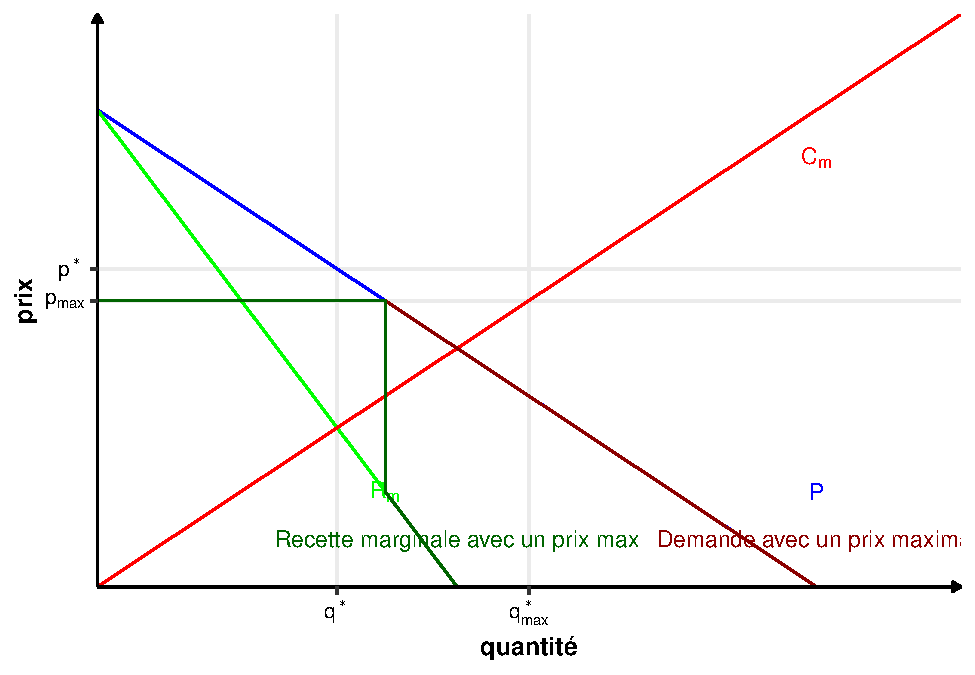
\includegraphics{_main_files/figure-latex/monopoleprixmaximal-1.pdf}
\caption{\label{fig:monopoleprixmaximal}Fixation d'un prix maximal supérieur au prix de CPP.}
\end{figure}

\begin{figure}
\centering
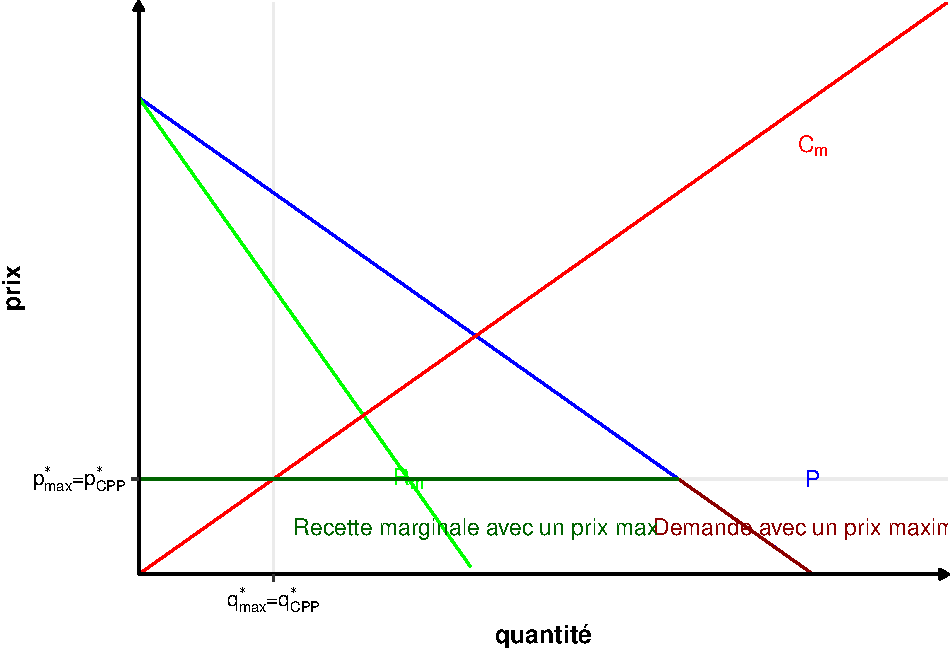
\includegraphics{_main_files/figure-latex/monopoleprixmaximal2-1.pdf}
\caption{\label{fig:monopoleprixmaximal2}Fixation d'un prix maximal inférieur au prix de CPP.}
\end{figure}

Si le prix maximum est inférieur au prix de concurrence pure et parfaite, les quantités produites peuvent devenir sous-optimale.
Le gouvernement peux maximiser le surplus social en prenant le prix concurrentiel comme prix maximum.\\
\emph{Rappel :} En CPP, on obtient le prix à l'aide de la courbe de coût marginal.
L'équilibre a lieu quand le coût marginal et la demande se croisent.

\begin{figure}
\centering
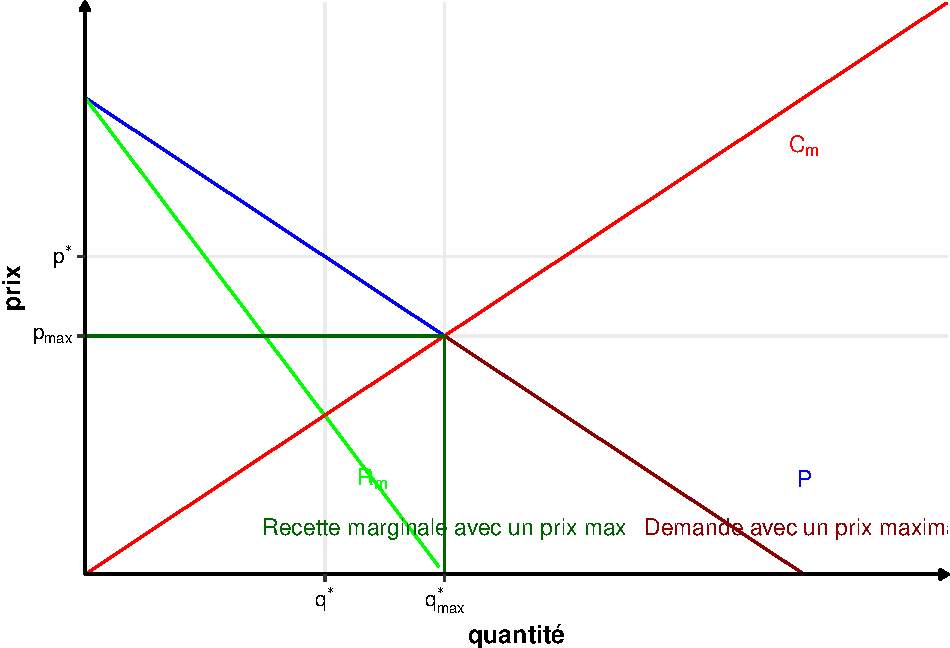
\includegraphics{_main_files/figure-latex/monopoleprixmaximalCPP-1.pdf}
\caption{\label{fig:monopoleprixmaximalCPP}Fixation d'un prix maximal égal au prix de CPP.}
\end{figure}

Avec un prix maximum égal au prix de concurrence pure et parfaite, le revenu marginal coupe la courbe de coût marginal au point d'équilibre de la concurrence pure et parfaite.

Globalement, si le prix maximal est entre le prix de monopole et le prix de concurrence pure et parfaite, alors la quantité produite augmente quand le prix maximal diminue.
Si au contraire le prix maximal est inférieur au prix de CPP (et donc de monopole), alors la quantité produite diminue quand le prix maximal augmente.

\hypertarget{le-monopole-naturel}{%
\section{Le monopole naturel}\label{le-monopole-naturel}}

Une situation de monopole naturel émerge à cause d'une structure particulière de la technologie de production et des coûts, plutôt qu'à cause d'une disposition légale.

\begin{definition}[Monopole naturel]
Un monopole naturel émerge en présence d'une technologie dotée de rendements d'échelles \emph{croissants} dans la zone de production optimale.
\end{definition}

Les rendements d'échelles sont croissants lorsque la technologie de production \(f\) est telle que :
\[
f(\lambda z_1, \lambda z_2, ...\lambda z_n) > \lambda f(z_1,z_2, ..., z_n)
\]
où les \(z_i\) sont les facteurs de productions.
En mots : une entreprise utilisant \(\lambda\) fois plus de facteurs de productions qu'une petite entreprise produit plus que \(\lambda\) petites entreprises réunies.

En général, un monopole naturel émerge à cause de coûts fixes élevés.
Par exemple, lorsqu'il faut investir dans un réseau (ferrés, téléphone, électricité, etc).

Une conséquence des rendements d'échelle croissants est que le coût moyen est décroissant :
\[
C_M(f(\lambda z)) =\frac{\lambda z\cdot w_z}{f(\lambda z)} < C_M(\lambda f(z)) = \frac{\lambda z\cdot w_z}{\lambda f(z)}
\]
car \(f(\lambda z)>\lambda f(z)\)
Cela signifie qu'une seule entreprise qui produit \(f(\lambda z)\) est plus efficace que \(\lambda\) entreprises qui produisent \(\lambda f(z)\).
Il y a ici des économies d'échelle.

\begin{definition}[Économie d'échelle]
Il y a des \emph{économies d'échelle} quand une unité de bien produite en plus revient moins chère que l'unité précédente.
Cela signifie que le \emph{coût moyen} baisse quand le producteur produit plus d'unités.
\end{definition}

De manière générale, il y a presque toujours une zone où le coût moyen est décroissant, mais elle est rarement très étendue.
Dans le graphique \ref{fig:monopolenaturelcout}, la demande inverse 1 coupe la courbe de coût marginal à un endroit où les économies d'échelle sont décroissantes.
La demande 2, en revanche, la coupe à un endroit où les économies d'échelle sont croissantes.

\begin{figure}
\centering
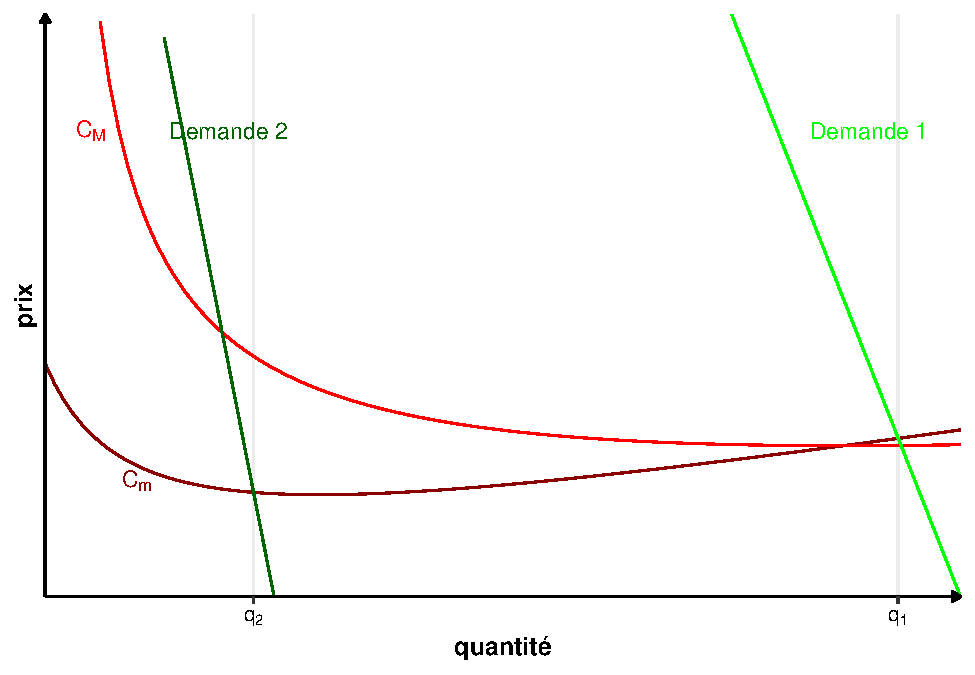
\includegraphics{_main_files/figure-latex/monopolenaturelcout-1.pdf}
\caption{\label{fig:monopolenaturelcout}Fonction de coût et demande avec et sans économies d'échelle.}
\end{figure}

\begin{remark}[Lien entre coût marginal et coût moyen en monopole naturel.]
Lorsque le coût moyen est décroissant, c'est que le coût marginal est inférieur au coût moyen.
\[
C_M(q) = \frac{C(q)}{q}
\]
\[
C_M'(q) =\frac{C'(q)q-C(q)}{q^2} = \frac{C_m(q)-C_M(q)}{q}
\]
Or \(C_M'(q)<0\), comme le coût marginal est décroissant.
On en déduit donc que
\[
C_m(q)-C_M(q)< 0 \Leftrightarrow C_m(q)<C_M(q)
\]
\end{remark}

\begin{remark}[Rendements d'échelle et économies d'échelle]
Il ne faut pas confondre les rendements d'échelle, qui mettent en relation les \textbf{quantités} de facteurs de productions et les quantités de biens produites et économies d'échelle, qui est une notion lié au \textbf{coût} de production des unités de biens produites.
\end{remark}

\textbf{Question :} Que se passe-t-il quand la fonction de demande inverse coupe la courbe de coût marginal dans la partie où le coût marginal est inférieur au coût moyen (où \(C_m<C_M\)) ?

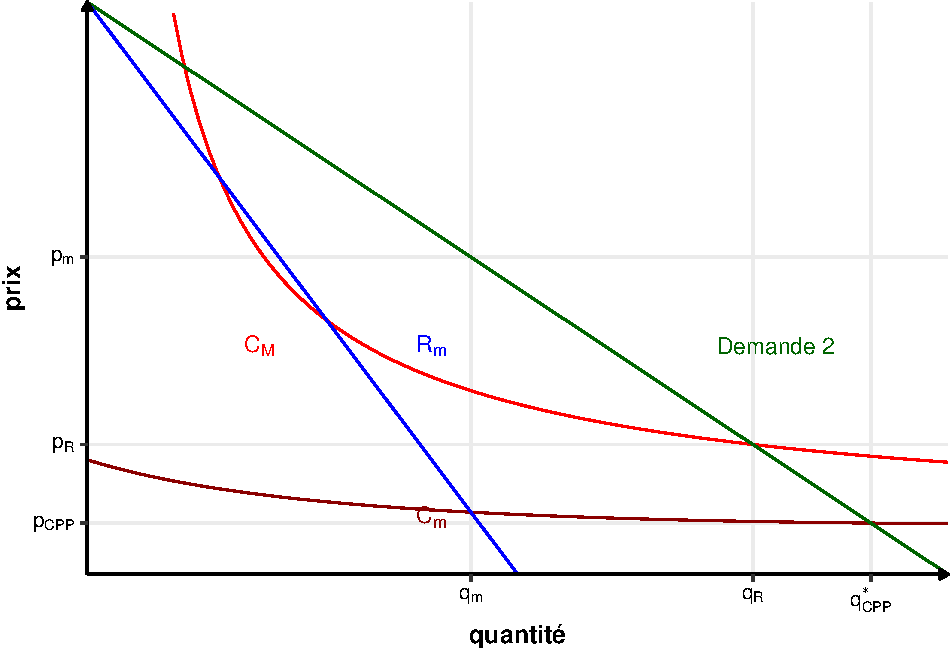
\includegraphics{_main_files/figure-latex/monopolenaturel-1.pdf}
Si on impose une tarification au coût marginal, alors le monopole fait des pertes, car le prix est inférieur au coût moyen.
La régulation ``optimale'' généralement utilisée impose \emph{un prix au coût moyen} et une obligation de satisfaire toute la demande.
Le monopole fait alors un profit nul.

Une solution alternative est un prix égal au coût moyen assorti de subventions pour couvrir les pertes.

\hypertarget{le-monopole-discriminant}{%
\section{Le monopole discriminant}\label{le-monopole-discriminant}}

Un monopole discriminant pratique un prix différent pour chaque (groupe de) consommateurs.
Pour cela, il doit pouvoir identifier l'appartenance de chaque consommateur à un groupe et les marchés entre les consommateurs doivent être hermétiques.
En particulier, il ne faut pas qu'un consommateur puisse revendre son unité de bien à un autre consommateur.

Il existe 3 types de discriminations par les prix, les discrimination du premier, deuxième et troisième degrés.
On ne traitera que les discriminations du premier et troisième degrés dans ce cours.

\hypertarget{discrimination-au-premier-degruxe9-discrimination-parfaite}{%
\subsection{Discrimination au premier degré (discrimination parfaite)}\label{discrimination-au-premier-degruxe9-discrimination-parfaite}}

Dans une discrimination parfaite, le monopole connaît la valorisation (prix de réserve) de chaque individu et lui fait payer le prix maximum qu'il est prêt à payer (son prix de réserve donc).
Le consommateur ne retient alors aucun surplus, la \emph{totalité} du surplus est capturé par le producteur.

\emph{Question :} Quel va être le niveau de production du monopole ?

Comme le monopole fait payer chaque unité à la valorisation du consommateur, la première unité est vendue au prix P(1), la deuxième au prix P(2), etc.
La recette totale est donc :
\[
R(q) = \int_0^q P(x) dx
\]
Notons le coût total \(C(q)\).
Le profit est :
\[
\pi(q) = R(q) - C(q) = \int_0^q P(x) dx -C(q)
\]
La condition du premier ordre s'écrit donc :
\[
\begin{array}{rl}
&\frac{d\pi(q^*)}{dq} = 0\\
\Leftrightarrow & \frac{d\int_0^{q^*} P(x) dx -C(q^*)}{dq} = 0\\
\Leftrightarrow & P(q^*) - C_m(q^*) = 0\\
\Leftrightarrow & P(q^*) = C_m(q^*)
\end{array}
\]
La recette marginale est ici confondue avec la courbe de demande.
L'optimum se trouve donc au point où la courbe de coût marginal coupe la courbe de demande (inverse).
C'est la même condition qu'en CPP.
Le monopole parfaitement discriminant produit donc la quantité de concurrence pure et parfaite.
Le prix de la dernière unité vendue par le monopole est égal au prix de la concurrence pure et parfaite, même si les prix des autres unités vendues sont supérieurs au prix de la CPP.

\begin{figure}
\centering
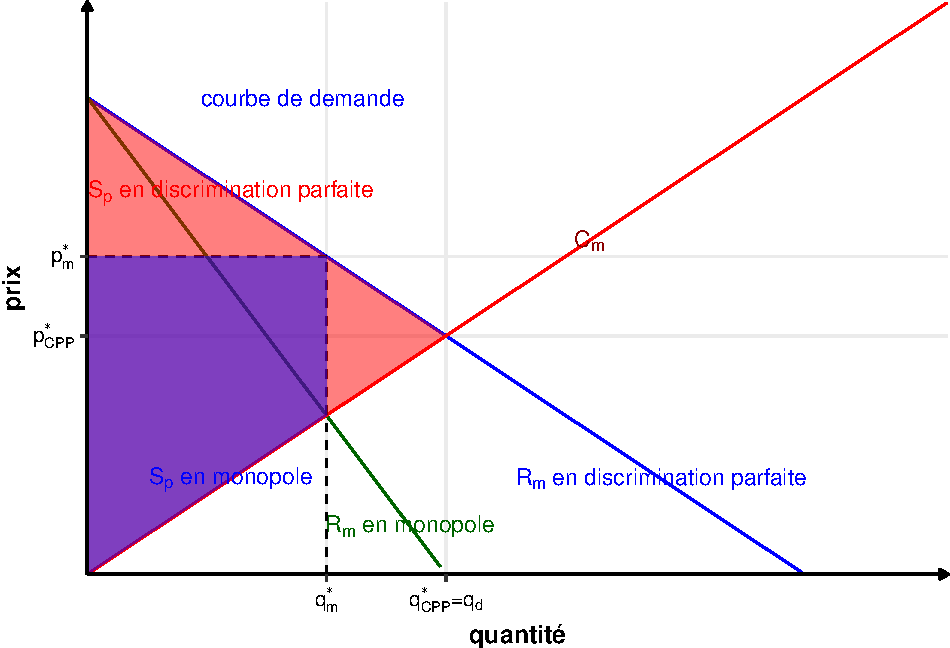
\includegraphics{_main_files/figure-latex/monopolediscriparfaite-1.pdf}
\caption{\label{fig:monopolediscriparfaite}Surplus du monopole en discrimination parfaite (aire rouge et bleue).}
\end{figure}

La situation de discrimination parfaite est un optimum de Pareto.
En effet, le surplus social est maximal (mais capturé entièrement par le monopole).

En pratique, il est très difficile de faire de la discrimination parfaite.
Les entreprises essaient de s'en approcher le plus possible.

Un exemple existe, lors d'une vente de bons du trésors des Etats-Unis.
Chaque ménage intéressé soumettait une offre (prix, quantité) au gouvernement.
Le gouvernement triait les offres par ordre décroissant de prix et les satisfait jusqu'à épuisement des bons à vendre.

\hypertarget{discrimination-du-deuxiuxe8me-degruxe9}{%
\subsection{Discrimination du deuxième degré}\label{discrimination-du-deuxiuxe8me-degruxe9}}

\begin{definition}[Discrimination du deuxième degré]
La discrimination du deuxième degré a lieu lorsque les prix de ventes dépendent des quantités achetées.
\end{definition}

Par exemple, si les 10 premières unités vendues le sont à 5€, et les suivantes à 2€.
Les prix de ventes sont nécessairement \emph{décroissants} avec la quantité vendue.

\begin{figure}
\centering
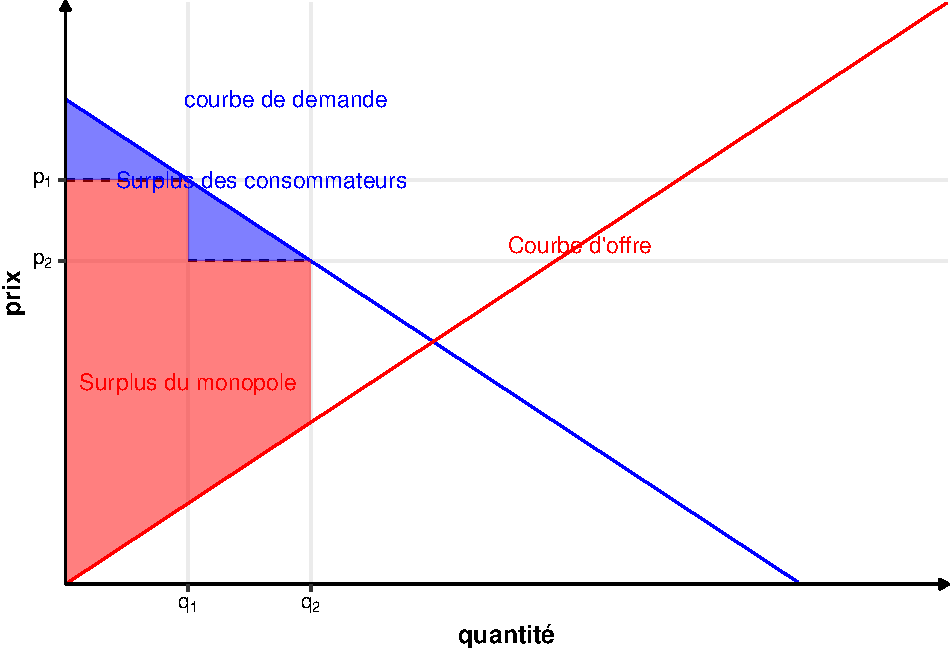
\includegraphics{_main_files/figure-latex/monopolediscri2degre-1.pdf}
\caption{\label{fig:monopolediscri2degre}Graphique avec une discrimination du deuxième degré. Les quantités inférieures à \(q_1\) sont vendues au prix \(p_1\), les suivantes au prix \(p_2\).}
\end{figure}

Le monopole ajuste les quantités seuils afin de maximiser son profit.
Il y a un nombre fini de seuils de dégressivité.
Plus il y a de seuils, plus on s'approche d'un situation de discrimination parfaite.

\hypertarget{discrimination-du-troisiuxe8me-degruxe9}{%
\subsection{Discrimination du troisième degré}\label{discrimination-du-troisiuxe8me-degruxe9}}

Il s'agit de faire payer un prix différent à chaque groupe de consommateur, en fonction des caractéristiques de leurs fonctions de demande.
Tous les membres d'un groupe payent donc le même prix, contrairement à la discrimination au premier degré.
Les groupes sont en général caractérisés par des propensions à payer différentes.
Il s'agit d'une segmentation des consommateurs.

\begin{example}[Discrimination au troisième degré]
Les tarifs jeunes de la SNCF, les tarifs familles.
Il est important de pouvoir identifier les groupes.
\end{example}

\emph{Question :} Comment répartir la production entre les différents groupes ?

\begin{enumerate}
\def\labelenumi{\arabic{enumi}.}
\tightlist
\item
  Quelle production totale ?
\item
  Quelle répartition ?
\end{enumerate}

\emph{Méthode :} On résout d'abord 2 en supposant que 1 est déjà résolu.
On obtient alors la répartition en fonction de la production totale.
Puis ou résout 1 à l'aide de la solution de 2.

On modélise le problème de la manière suivante :

\begin{itemize}
\tightlist
\item
  2 groupes A et B;
\item
  Avec des fonctions de demande inverses \(P_A(q_A)\) et \(P_B(q_B)\);
\item
  Une quantité \(q\) totale a été produite, qu'il faut répartir entre les 2 groupes : \(q=q_A+q_B\)
\end{itemize}

Le problème du monopole s'écrit :
\[
\max_{q_A, q_B} \pi(q_A, q_B) = q_AP_A(q_A) + q_BP_B(q_B) -C(q)
\]
La quantité totale \(q\) est fixée, donc le coût total l'est aussi et peut être supprimé du problème de maximisation.
On cherche donc juste à maximiser la recette totale :
\[
\max_{q_A, q_B} q_AP_A(q_A) + q_BP_B(q_B) 
\]
Avec \(q=q_A+q_B\), donc \(q_B=q-q_A\), le problème devient :
\[
\begin{array}{rl}
&\max_{q_A, 0\leq q_A\leq q} q_AP_A(q_A) + (q-q_A)P_B(q-q_A) \\
\Leftrightarrow &\max_{q_A, 0\leq q_A\leq q} R_A(q_A) + R_B(q-q_A) 
\end{array}
\]
La condition du premier ordre s'écrit :
\[
\begin{array}{rl}
&\frac{dR_A(q_A) + R_B(q-q_A) }{dq_A} = 0\\
\Leftrightarrow & R_{mA}(q_A) - R_{mB}(q-q_A) = 0\\
\Leftrightarrow & R_{mA}(q_A) = R_{mB}(q_B) 
\label{eq:cpo3e}
\end{array}
\]
L'équation \eqref{eq:cpo3e} nous dit que le monopole réparti la quantité totale produite de manière égaliser les recettes marginales entre les deux groupes.

Intuitivement, si la recette marginale issue du groupe A est supérieure à celle issue du groupe B (\(R_{mA}(q_A) > R_{mB}(q_B)\)), alors en diminuant la quantité \(q_B\) dans le groupe B et en la transférant au groupe A, le monopole perd \(R_{mB}(q_B)\) et gagne \(R_{mA}(q_A)\), donc la recette totale augmente et le profit aussi.
Inversement dans le cas opposé.
Il n'est donc pas intéressant de transférer la production d'un groupe vers un autre lorsque \(R_{mA}(q_A) = R_{mB}(q_B)\) (et seulement dans ce cas).

Maintenant que la répartition est résolue, il faut trouver la quantité totale produite.
Le problème devient maintenant :
\[
\max_{q_A, q_B} \pi(q_A, q_B) = q_AP_A(q_A) + q_BP_B(q_B) -C(q_A+q_B)
\]
La condition du premier ordre s'obtient maintenant en dérivant suivant \(q_A\) et \(q_B\) séparément :
\[
\begin{array}{rcl}
\frac{\partial\pi(q_A, q_B)}{\partial q_A} = 0&\Leftrightarrow& R_{mA}(q_A^*) = C_m(q_A^*+q_B^*)\\
\frac{\partial\pi(q_A, q_B)}{\partial q_B} = 0&\Leftrightarrow& R_{mB}(q_B^*) = C_m(q_A^*+q_B^*)\\
\end{array}
\]
Le monopole doit faire en sorte que le coût marginal de sa production totale soit égale à la recette marginale sur chacun des marchés.

\emph{Intuition :}
Le monopole doit égaliser la recette marginale sur les deux marchés.
Or le coût marginal dépend de la quantité \emph{totale} produite, pas de la répartition entre les marchés.
Si on est dans la situation telle que \(C_m(q)<R_{mA}(q_A)\), alors il y a la possibilité de faire du profit sur le marché A (et le marché B par conséquent).
Inversement, si \(C_m(q)>R_{mA}(q_A)\), alors le monopole fait des pertes.

\begin{remark}
On utilise bien \(C_m(q_A+q_B)\) et non \(C_m(q_A)\) ou \(C_m(q_B)\) car c'est bien la variation du coût total lorsqu'on augmente ``un peu'' \(q_A\) et \(q_B\) reste fixe.
\end{remark}

D'après l'équation \eqref{eq:rm}, on peut écrire :
\[
\begin{array}{crcl}
&R_{mA}(q_A^*) &=& R_{mB}(q_B^*)\\
\Leftrightarrow & P_A(q_A^*)\left(1-\frac{1}{\left|\varepsilon_{q/p_A}(q^*_A)\right|}\right) & = & P_B(q_B^*)\left(1-\frac{1}{\left|\varepsilon_{q/p_B}(q_B^*)\right|}\right)
\end{array}
\]
Sans perte de généralité, on peut supposer que \(P_A(q_A^*)> P_B(q_B^*)\).
On obtient alors que :
\[
1-\frac{1}{\left|\varepsilon_{q/p_A}(q_A^*)\right|} <1-\frac{1}{\left|\varepsilon_{q/p_B}(q_B^*)\right|}
\]
Autrement dit
\[
\left|\varepsilon_{q/p_B}(q_B^*)\right|>\left|\varepsilon_{q/p_A}(q^*_A)\right|
\]
Le prix est donc plus faible pour le groupe où l'élasticité prix de la demande est plus élevée.
Le prix est plus élevé pour le groupe avec l'élasticité la plus faible, les moins réactifs au prix.

\begin{example}
Les tarifs ``professionnels'' dans les transports (avion, train, etc).
Les professionnels sont moins sensibles au prix car leurs dates de voyage sont moins flexibles que celles des particuliers.
Leur élasticité prix est donc plus faible et leur prix plus élevés.
\end{example}

Des fonctions de demande inverse différentes associées à des élasticités prix de la demande différente aboutissent à des prix différents.

\hypertarget{oligopoles}{%
\chapter{Oligopoles}\label{oligopoles}}

On a vu jusqu'à présent deux cas extrêmes :

\begin{itemize}
\tightlist
\item
  La concurrence pure et parfaite :
  il y a une infinité d'entreprise infinitésimales sur un marché donné ;
\item
  Le monopole : il y a une seule entreprise sur un marché donné.
\end{itemize}

Dans les deux cas, le ou les entreprises n'ont pas à se préoccuper des autres entreprises.
Dans le cas du monopole, parce qu'il n'y en a pas.
Dans le cas de la CPP, l'entreprise observe le prix du marché et prend sa décision en fonction de ce prix, et uniquement de ce prix.
Les actions des autres entreprises ne l'influence pas.

On considère maintenant la situation où il n'y a plus une seule ou une infinité d'entreprises, mais plusieurs, qui sont en situation d'\emph{interactions stratégiques}.
Les décisions de chaque acteur dépend des décisions des autres acteurs (ou des anticipations de ces décisions).\\
On parle de \emph{duopole} dans le cas où le marché compte deux entreprises et d'\emph{oligopole} dans le cas où il compte plus que deux entreprises.\\
Les entreprises peuvent se faire concurrence de différentes manières :

\begin{itemize}
\tightlist
\item
  En quantité, concurrence dite à la \emph{Cournot} ;
\item
  En prix, concurrence à la \emph{Bertrand} ;
\item
  En prenant une situation de leader ou de follower, à la \emph{Stackelberg} ;
\item
  En format une entente, dans un \emph{cartel} ;
\item
  Dans une concurrence spatiale, à la \emph{Hotelling}.
\end{itemize}

Nous verrons dans ce cours les concurrences à la Cournot et à la Stackelberg, ainsi que les cartels.

\hypertarget{duopole-uxe0-la-cournot}{%
\section{Duopole à la Cournot}\label{duopole-uxe0-la-cournot}}

\hypertarget{introduction}{%
\subsection{Introduction}\label{introduction}}

On considère deux entreprises sur le même marché qui doivent choisir les quantités à produire, sans connaître la quantité choisie par l'autre (= décision simultanée).\footnote{Même marché : bien unique et prix unique.}
Le prix est déterminé par la quantité \emph{totale} produite par les deux entreprises et la fonction de demande sur le marché.

Chaque entreprise est caractérisée par une quantité produite et un coût :

\begin{itemize}
\tightlist
\item
  Entreprise 1 : quantité \(q_1\) produite au coût \(C_1(q_1)\) ;
\item
  Entreprise 2 : quantité \(q_2\) produite au coût \(C_2(q_2)\).
\end{itemize}

Les fonctions de coût sont \textbf{différentes} entre les deux entreprises, contrairement au cas du monopole discriminant au troisième degré, où l'on considérait \(C(q_1+q_2)\).

La fonction de demande inverse sur le marché est \(P(q_1+q_2)\).
C'est différent du monopole discriminant où il y avait une fonction de demande par segment.

On a donc les fonctions de profit:
\[
\begin{array}{rcl}
\pi_1(q_1, q_2) &=& P(q_1+q_2)\cdot q_1-C_1(q_1)\\
\pi_2(q_1, q_2) &=& P(q_1+q_2)\cdot q_2-C_2(q_2)
\end{array}
\]
L'action d'une entreprise a des conséquences sur le profit réalisé par l'autre entreprise, même si celle-ci ne fait rien.
En particulier, si \(q_1\) augmente, alors le prix du marché diminue, au travers de la fonction de demande inverse \(P\), et donc le profit de l'entreprise 2, \(\pi_2\), diminue, et réciproquement si \(q_2\) augmente.
Il y a donc un conflit d'intérêt entre les producteurs.
Chaque entreprise doit anticiper l'action de l'autre et réagir à cette anticipation le mieux possible.

\emph{Question :} Peut-il y avoir un équilibre dans cette situation ?

\hypertarget{formalisation-du-probluxe8me}{%
\subsection{Formalisation du problème}\label{formalisation-du-probluxe8me}}

\hypertarget{expression-des-profits}{%
\subsubsection{Expression des profits}\label{expression-des-profits}}

On a des profits :
\[
\begin{array}{rcl}
\pi_1(q_1, q_2) &=& P(q_1+q_2)\cdot q_1-C_1(q_1)\\
\pi_2(q_1, q_2) &=& P(q_1+q_2)\cdot q_2-C_2(q_2)
\end{array}
\label{eq:profitcournot}
\]

Supposons que l'entreprise 1 \emph{croit} que l'entreprise 2 va produire \(q_2^a\).
Quelle est sa production optimale ?
Son problème de maximisation est :
\[
\max_{q_1} \pi_1(q_1, q_2^a) =  q_1P(q_1+q_2^a)-C_1(q_1)
\]
On peut déduire de ce problème d'optimisation la \emph{fonction de réaction} \(q_1(q_2^a)=f_1(q_2^a)\) qui maximise \(\pi_1(q_1)\) en fonction de la production anticipée \(q_2^a\) de l'entreprise 2.\footnote{La fonction de réaction est parfois aussi connue sous le nom de \emph{fonction de meilleure réponse}.}
La fonction de réaction \(f_1(q_2^a)\) donne la valeur de \(q_1\) qui maximise le profit quand l'entreprise 2 produit \(q_2^a\).

De la même manière, l'entreprise 2 cherche à maximiser \(\pi_2\) en fonction de la production anticipée \(q_1^a\) de l'entreprise 1.
Son programme est :
\[
\max_{q_2} \pi_2(q_1^a, q_2) =  q_1P(q_1^a+q_2)-C_2(q_2)
\]
Elle aura également une fonction de réaction \(q_2(q_1^a)=f_2(q_1^a)\).

\hypertarget{forme-des-fonctions-de-ruxe9action}{%
\subsubsection{Forme des fonctions de réaction}\label{forme-des-fonctions-de-ruxe9action}}

Si l'entreprise \(i\) pense que l'entreprise \(j\) ne va rien produire, alors elle se trouve dans une situation de monopole et se comporte comme tel.
Elle produit de manière à égaliser coût marginal et recette marginale (\(R_{im}=C_{im}\)).

Si l'entreprise \(i\) pense que l'entreprise \(j\) va produire \(q_j^a>0\), alors elle est en monopole sur le \textbf{reste} de la demande.
Cette dernière correspond à la demande totale décalée de \(q_j^a>0\) vers la gauche.
Le croisement entre recette marginale et coût marginal se fait donc à un niveau plus faible qu'auparavant.

Plus l'entreprise \(i\) pense que l'entreprise \(j\) va produire une grande quantité, plus elle aura intérêt à réduire son offre.
\(q_i\) est décroissante en \(q_j^a\)

\begin{figure}
\centering
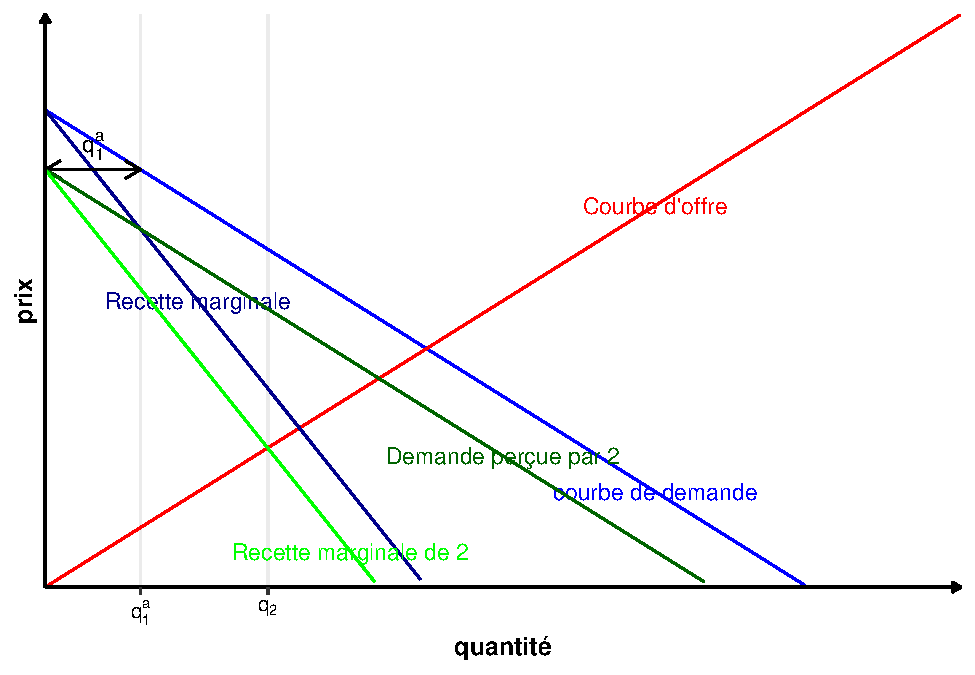
\includegraphics{_main_files/figure-latex/oligodemande-1.pdf}
\caption{\label{fig:oligodemande}Représentation de la demande perçue par l'entreprise 2 anticipant une offre \(q_1^a\) par l'entreprise 1.}
\end{figure}

\hypertarget{caractuxe9risation-de-luxe9quilibre}{%
\subsubsection{Caractérisation de l'équilibre}\label{caractuxe9risation-de-luxe9quilibre}}

Un équilibre \((q_1^a, q_2^a)\) doit être tel qu'aucune des deux entreprises n'ait intérêt à dévier unilatéralement :
\[
\begin{array}{rcl}
\pi_1(q_1^a, q_2^a) &\geq& \pi_1(q_1, q_2^a)\quad \forall q_1\\
\pi_2(q_1^a, q_2^a) &\geq& \pi_2(q_1^a, q_2)\quad \forall q_2
\end{array}
\]
Au point \(q_1^a\) et \(q_2^a\), aucune entreprise n'a intérêt à dévier unilatéralement de l'équilibre.
Les décisions prises sont mutuellement compatibles.
Chaque entreprise donne sa meilleure réponse à la meilleure réponse de l'autre.
C'est ce qu'on appelle un \textbf{équilibre de Nash} : un équilibre où personne n'a intérêt à dévier unilatéralement.

Dans le cas du duopole à la Cournot, chaque entreprise doit choisir la quantité qui maximise son profit étant donné le choix de l'autre entreprise.
Chaque entreprise est donc sur sa fonction de réaction.
L'équilibre est donc à l'intersection des fonctions de réactions des deux entreprises :
\[
\begin{array}{rcl}
q_1^a&=&f_1(q_2^a)\\
q_2^a&=&f_2(q_1^a)
\end{array}
\]

\begin{figure}
\centering
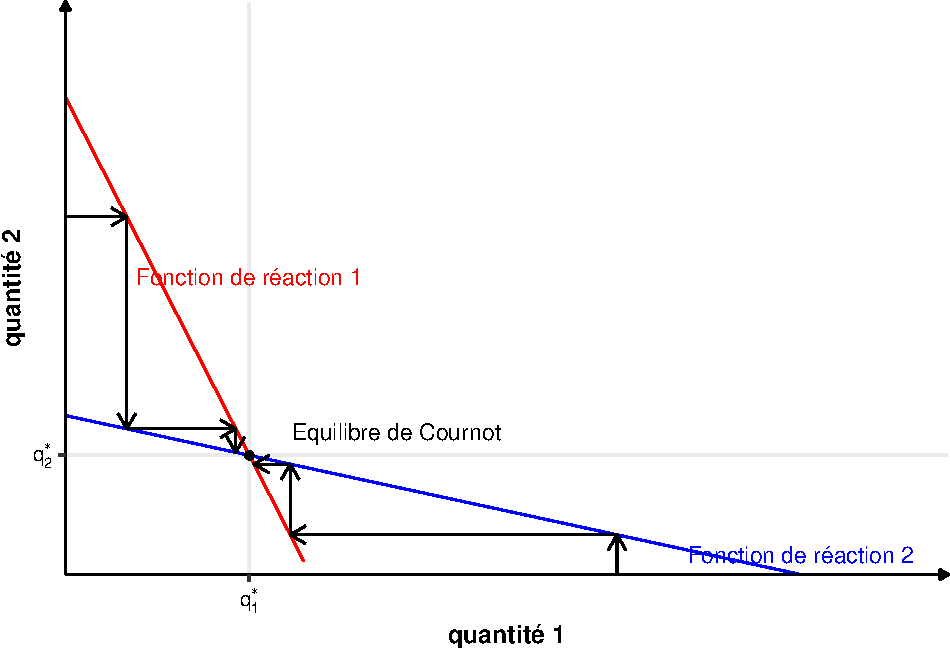
\includegraphics{_main_files/figure-latex/oligoreaction-1.pdf}
\caption{\label{fig:oligoreaction}Représentation d'un équilibre de Cournot où les fonctions de réaction convergent vers le point d'équilibre.}
\end{figure}

L'équilibre n'est pas nécessairement stable.
La stabilité dépend de la pente des fonctions de réactions.

\begin{figure}
\centering
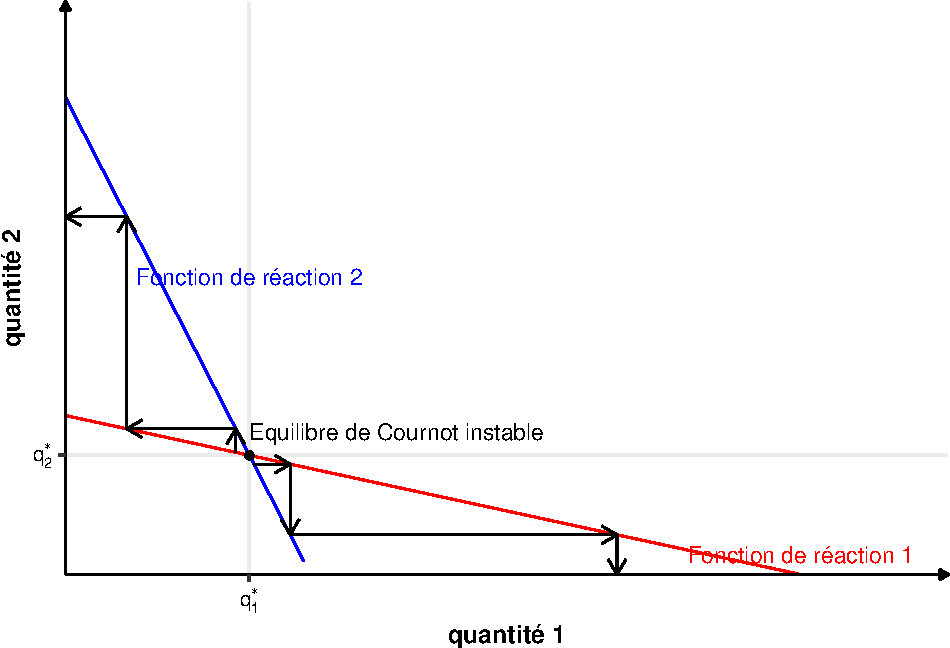
\includegraphics{_main_files/figure-latex/oligoreactioninstable-1.pdf}
\caption{\label{fig:oligoreactioninstable}Représentation d'un équilibre de Cournot où les fonctions de réaction divergent du point d'équilibre. Equilibre instable}
\end{figure}

\hypertarget{exemple}{%
\subsection{Exemple}\label{exemple}}

\hypertarget{donnuxe9es-du-probluxe8me}{%
\subsubsection{Données du problème}\label{donnuxe9es-du-probluxe8me}}

Prenons les fonctions suivantes :

\[
\begin{array}{l}
P(q_1+q_2) = a - b(q_1+q_2)\\
C_1(q_1) = cq^2_1 \\
C_2(q_2) = cq^2_2 \\
\end{array}
\]

\hypertarget{profits}{%
\subsubsection{Profits}\label{profits}}

On en déduit les profits :

\[
\begin{array}{rcl}
\pi_1(q_1, q_2) &=& \left(a-b(q_1+q_2)\right)q_1-cq_1^2\\
\pi_2(q_1, q_2) &=& \left(a-b(q_1+q_2)\right)q_2-cq_2^2
\end{array}
\]

\hypertarget{fonctions-de-ruxe9action}{%
\subsubsection{Fonctions de réaction}\label{fonctions-de-ruxe9action}}

Calculons la fonction de réaction de l'entreprise 1.
Son profit est :
\[
\pi_1(q_1, q_2^a) = aq_1-bq_1^2-bq_2^aq_1-cq_1^2 = (a-bq_2^a)q_1-(b+c)q_1^2
\]

La condition du premier ordre suivant \(q_1\) s'écrit (ici \(q_2^a\) est considéré comme une donnée par l'entreprise 1) :

\[
\begin{array}{crcl}
&\frac{\partial \pi_1}{\partial q_1}&=&0\\
\Leftrightarrow & (a-bq_2^a)-2(b+c)q_1^* &=& 0\\
\Leftrightarrow & q_1^* &=& \frac{(a-bq_2^a)}{2(b+c)}
\label{eq:FR1}
\end{array}
\]

On calcule de la même manière (i.e., en utilisant la condition du premier ordre sur les profits de l'entreprise 2) la fonction de réaction de l'entreprise 2 et on obtient par symétrie du problème une légère réécriture de l'équation \eqref{eq:FR1}:

\[
q_2^* = \frac{(a-bq_1^a)}{2(b+c)}
\]

La symétrie du problème provient du fait que les deux entreprises ont exactement la même fonction de coût.
Ce \emph{n'est pas le cas en général}.
Si dans un problème les fonctions de coût sont identiques, alors vous pouvez faire les calculs pour une seule entreprise et déduire simplement les résultats pour la seconde.

\hypertarget{equilibre-de-cournot}{%
\subsubsection{Equilibre de Cournot}\label{equilibre-de-cournot}}

Quel est alors l'équilibre de Cournot ?

On doit avoir :
\[
\begin{array}{rcl}
f_1(q_2^*) &=& q_1^*\\
f_2(q_1^*) &=& q_2^*\\
\end{array}
\]
Autrement dit :
\[
\begin{array}{rcl}
q_1^* &=& \frac{(a-bq_2^*)}{2(b+c)} \\
q_2^* &=&\frac{(a-bq_1^*)}{2(b+c)}\\
\end{array}
\]
On résout le système et on obtient :
\[
q_1^*=q_2^* = \frac{a}{3b+2c}
\]

Quand le problème est symétrique, les deux entreprises en compétition à la Cournot produisent la même quantité de bien.

\hypertarget{une-intuition-graphique-les-courbes-disoprofit}{%
\subsection{Une intuition graphique : les courbes d'isoprofit}\label{une-intuition-graphique-les-courbes-disoprofit}}

On peut aussi aborder le problème à l'aide d'une intuition graphique.
Il s'agit de tracer les courbes d'\emph{isoprofit} des entreprises.

\begin{definition}[Courbe d'isoprofit]
Les courbes d'isoprofit est l'ensemble des couples de quantités \((q_1, q_2)\) qui permettent à une entreprise d'atteindre un niveau de profit donné.
\end{definition}

Reprenons l'expression générale des profits de l'équation \eqref{eq:profitcournot}.
\[
\begin{array}{rcl}
\pi_1(q_1, q_2) &=& q_1P(q_1+q_2)-C_1(q_1)\\
\pi_2(q_1, q_2) &=& q_2P(q_1+q_2) -C_2(q_2)
\end{array}
\]
La courbe d'isoprofit pour une valeur \(\pi_1\) \textbf{donnée et fixe} est :
\[
\pi_1 = q_1P(q_1+q_2)-C_1(q_1)
\]
L'équation ci-dessus définit implicitement une fonction \(q_1=I_\pi(q_1, \pi_1)\) qui permet de représenter la courbe d'isoprofit dans un graphique \((q_1,q_2)\), tout comme la fonction de réaction définit une fonction courbe \(q_2(q_1)\) pour l'entreprise 1.
La courbe de la fonction de réaction de 1 coupe la courbe d'isoprofit de 1 en son maximum.

\begin{figure}
\centering
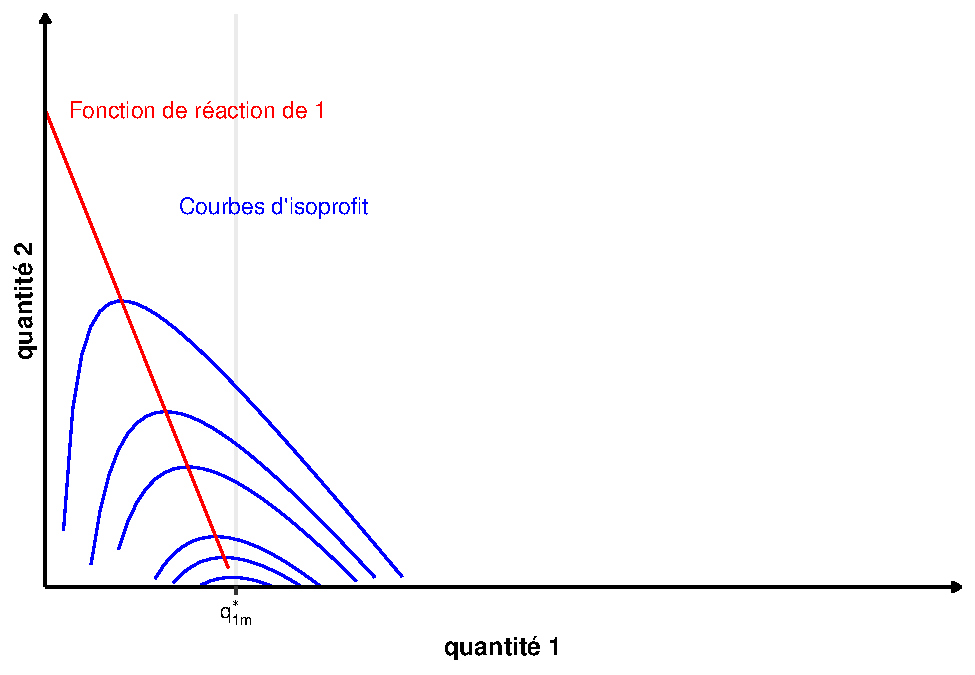
\includegraphics{_main_files/figure-latex/isoprofit1-1.pdf}
\caption{\label{fig:isoprofit1}Courbes d'isoprofit et fonction de réaction de l'entreprise 1}
\end{figure}

Sur la figure \ref{fig:isoprofit1}, le profit est croissant en descendant vers le bas sur les courbes d'isoprofit, autrement dit, les courbes d'isoprofit les plus basses représentent les profits les plus élevés.
Le maximum du profit est atteint lorsque l'entreprise 1 est en monopole.
La quantité produite est alors \(q_m^*\) est le profit \(\pi_m^*\).

\begin{figure}
\centering
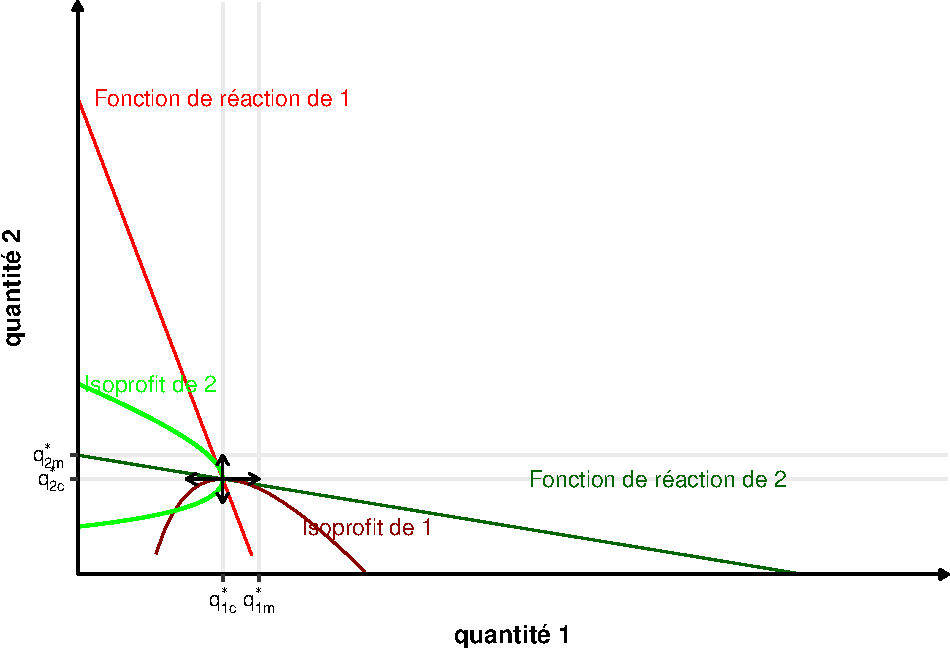
\includegraphics{_main_files/figure-latex/isoprofitCournot-1.pdf}
\caption{\label{fig:isoprofitCournot}Courbes d'isoprofits et fonctions de réactions des entreprises en équilibre de Cournot Nash.}
\end{figure}

\hypertarget{duopole-uxe0-la-stackelberg}{%
\section{Duopole à la Stackelberg}\label{duopole-uxe0-la-stackelberg}}

\hypertarget{introduction-1}{%
\subsection{Introduction}\label{introduction-1}}

Il n'y a plus de symétrie des entreprises dans un duopole à la Stackelberg.
Une entreprise, dite \emph{leader}, prend ses décisions avant l'entreprise dite \emph{follower}.
L'entreprise leader connaît les caractéristiques de l'entreprise follower et peut ainsi calculer sa fonction de réaction.
Elle en tiendra compte dans ses décisions.
On considère ici qu'il n'y a que deux périodes de décisions.

\hypertarget{ruxe9solution-graphique}{%
\subsection{Résolution graphique}\label{ruxe9solution-graphique}}

Le leader doit choisir sa quantité \(q_1\) de façon à être sur la courbe d'isoprofit la plus basse possible compatible avec la fonction de réaction de l'entreprise follower.
Il va donc se placer sur la courbe d'isoprofit tangente à la fonction de réaction du follower.

\begin{figure}
\centering
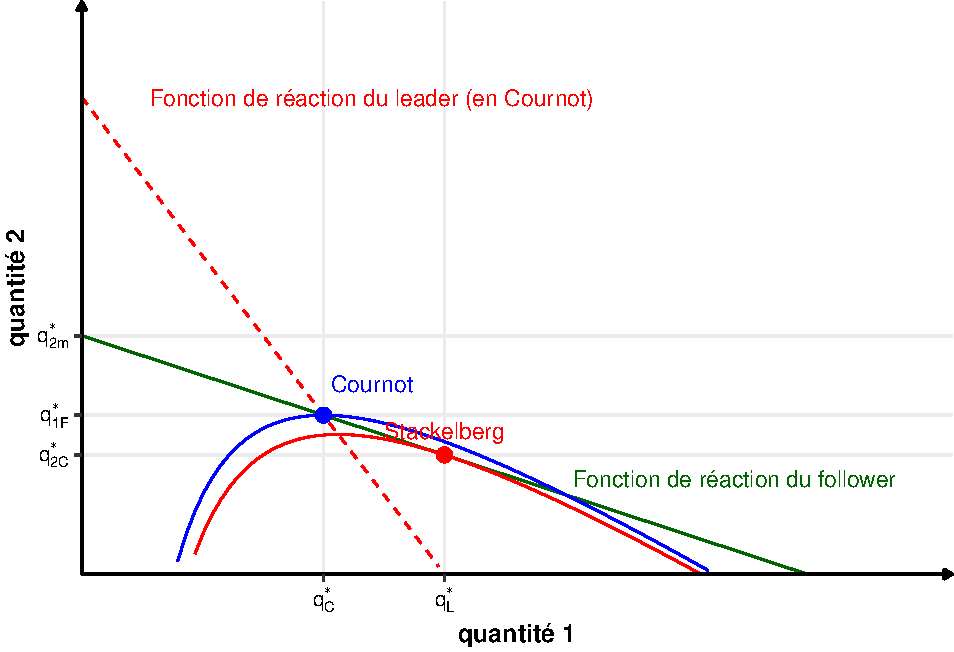
\includegraphics{_main_files/figure-latex/equilibreStackelberg-1.pdf}
\caption{\label{fig:equilibreStackelberg}Courbes d'isoprofits du leader et fonctions de réactions des entreprises en équilibre de Stackelberg.}
\end{figure}

Sur la figure \ref{fig:equilibreStackelberg}, on voit que le profit du leader est plus important en Stackelberg qu'en Cournot (et l'inverse pour le follower).
Les quantités produites par l'entreprise leader sont plus importantes en Stackelberg qu'en Cournot, mais celles du follower sont plus faibles.
La somme des deux est plus importante (\(q_{1C}^*+q_{2C}^*<q_{L}^*+q_{F}^*\)).
Le prix sera donc plus faible pour les consommateurs.

\hypertarget{exemple-1}{%
\subsection{Exemple}\label{exemple-1}}

\hypertarget{donnuxe9es-du-probluxe8mes}{%
\subsubsection{Données du problèmes}\label{donnuxe9es-du-probluxe8mes}}

Notons les variables et fonctions du leader avec un indice \(L\) et celles du follower avec un indice \(F\).

Gardons une fonction de demande linéaire.

\[
P(q_L+q_F) = a - b(q_L+q_F)
\]

Supposons, afin de simplifier les calculs, que les coûts marginaux sont nuls.

\hypertarget{profits-1}{%
\subsubsection{Profits}\label{profits-1}}

On en déduit les profits :

\[
\begin{array}{rcl}
\pi_L(q_L, q_F) &=& \left(a-b(q_L+q_F)\right)q_L\\
\pi_F(q_L, q_F) &=& \left(a-b(q_L+q_F)\right)q_F
\end{array}
\]

\hypertarget{fonction-de-ruxe9action-de-lentreprise-follower}{%
\subsubsection{Fonction de réaction de l'entreprise follower}\label{fonction-de-ruxe9action-de-lentreprise-follower}}

Calculons la fonction de réaction de l'entreprise follower.
La condition du premier ordre suivant \(q_F\) s'écrit (ici \(q_L\) est considéré comme une donnée par l'entreprise 1) :

\[
\begin{array}{crcl}
&\frac{\partial \pi_F}{\partial q_F}&=&0\\
\Leftrightarrow & (a-bq_L)-2bq_F^* &=& 0\\
\Leftrightarrow & q_F^* &=& \frac{a-bq_L}{2b}
\label{eq:FRFollower}
\end{array}
\]

\hypertarget{maximisation-de-lentreprise-leader}{%
\subsubsection{Maximisation de l'entreprise leader}\label{maximisation-de-lentreprise-leader}}

Comme l'entreprise leader connaît la fonction de réaction de l'entreprise follower (donnée par l'équation \eqref{eq:FRFollower}), elle peut l'intégrer à sa propre fonction de profit :

\[
\begin{array}{rcl}
\pi_L(q_L, q_F^*) &=& \left(a-b(q_L+q_F^*(q_L))\right)q_L\\
 &=& \left(a-b\left(q_L+\frac{a-bq_L}{2b}\right)\right)q_L\\
 &=& \frac{a}{2}q_L-\frac{b}{2}q_L^2
\end{array}
\]

La condition de premier ordre du leader est :

\[
\begin{array}{crcl}
&\frac{\partial \pi_L}{\partial q_L}&=&0\\
\Leftrightarrow & \frac{a}{2}-bq_L^* &=& 0\\
\Leftrightarrow & q_L^* &=& \frac{a}{2b}
\end{array}
\]

On en déduit qu'à l'équilibre de Stackelberg, le follower produit :
\[
q_F^*=\frac{a}{4b}
\]

L'entreprise leader produit plus que l'entreprise follower.
Elle profite de son pouvoir sur la seconde entreprise pour cela.
Si on calcule le profit, on verra que le profit de l'entreprise leader est plus important que celui de l'entreprise follower si elles sont exactement symétriques, en dehors de leur prises de décisions.

\hypertarget{cartels-et-collusions}{%
\section{Cartels et collusions}\label{cartels-et-collusions}}

\hypertarget{introduction-2}{%
\subsection{Introduction}\label{introduction-2}}

En duopoles / oligopoles de Cournot ou de Stackelberg, les entreprises ne coopèrent pas entre elles :

\begin{itemize}
\tightlist
\item
  Elles sont en concurrence ;
\item
  Elles agissent indépendamment les unes des autres.
\end{itemize}

\emph{Question :}\\
Que se passe-t-il si elles peuvent s'entendre ?
Par exemple, que se passe-t-il si elle peuvent passer un accord sur la quantité à produire.

\emph{Résultats :}\\
Les quantités mises sur le marché vont diminuer, et le prix du marché va augmenter.
C'est donc néfaste pour les consommateurs.
La raison est que le cartel se comporte exactement comme un monopole, puis partage les bénéfices.

\hypertarget{raisonnement-graphique}{%
\subsection{Raisonnement graphique}\label{raisonnement-graphique}}

\begin{figure}
\centering
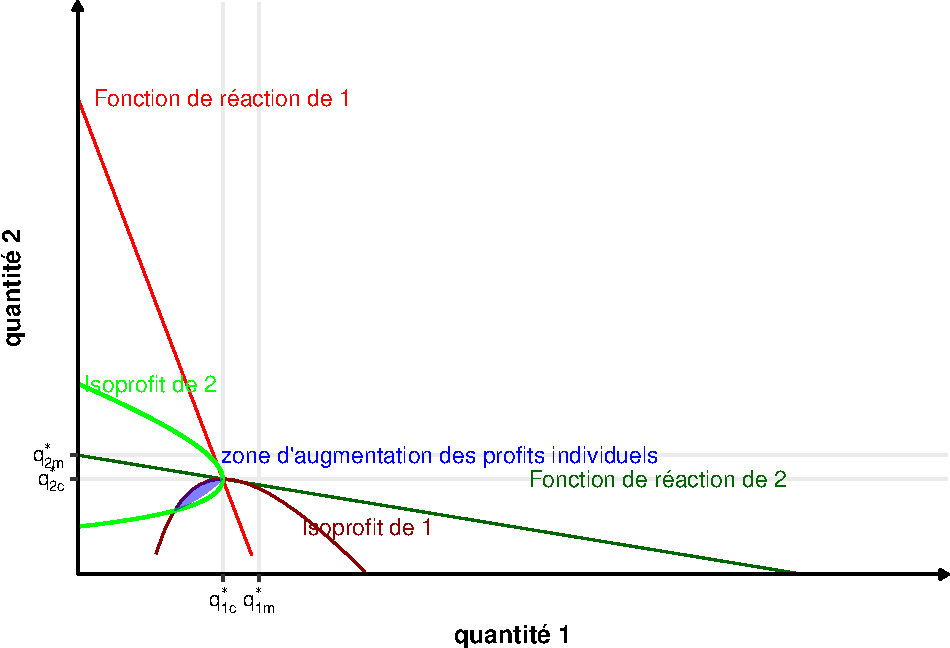
\includegraphics{_main_files/figure-latex/cartel-1.pdf}
\caption{\label{fig:cartel}Zone d'amélioration mutuellement bénéfique.}
\end{figure}

\hypertarget{ruxe9solution-analytique}{%
\subsection{Résolution analytique}\label{ruxe9solution-analytique}}

\hypertarget{iduxe9e}{%
\subsubsection{Idée}\label{iduxe9e}}

L'idée derrière la résolution analytique du problème du cartel est de considérer que le cartel se comporte comme un monopole avec 2 centres de productions.
Le cartel choisit la quantité globale produite et la répartition entre les entreprises.
C'est un raisonnement très similaire à un monopole discriminant au troisième degré.

\hypertarget{profits-2}{%
\subsubsection{Profits}\label{profits-2}}

Le profit global du cartel s'écrit :
\[
\pi_c=qP(q)-C_A(q_A)-C_B(q_B)=(q_A+q_B)P(q_A+q_B)-C_A(q_A)-C_B(q_B)
\]
Où \(q=q_A+q_B\).
Le profit est maximisé lorsque les dérivées partielles suivant chacune des quantités sont nulles (condition du premier ordre), c'est-à-dire lorsque \(\frac{\partial\pi_C}{\partial q_A}=0\) et \(\frac{\partial\pi_C}{\partial q_B}=0\).
\[
\frac{\partial\pi_C}{\partial q_A} = P(q) + q\frac{\partial P}{\partial q}(q_A)-\frac{\partial C_A}{\partial q_A}(q_A)
\]
On a \(P(q) + q\frac{\partial P}{\partial q}=R_m(q)\) est la recette marginale totale du cartel.
\(\frac{\partial C_A}{\partial q_A}=C_{mA}\) est le coût marginal de l'entreprise A.\\
On peut réécrire la dérivée du profit total suivant la quantité produite par l'entreprise A :
\[
\frac{\partial\pi_C}{\partial q_A} = R_m(q)  - C_{mA}(q_A)
\]
En utilisant le même raisonnement, on a pour l'entreprise B :
\[
\frac{\partial\pi_C}{\partial q_B} = R_m(q)  - C_{mB}(q_B)
\]

\hypertarget{optimalituxe9-pour-le-cartel}{%
\subsubsection{Optimalité pour le cartel}\label{optimalituxe9-pour-le-cartel}}

À l'optimum pour le cartel, on a donc :
\[R_m(q) = C_{mA}(q_A) = C_{mB}(q_B)\]
Le cartel égalise la recette marginale \emph{totale} aux coûts marginaux de chacune des deux entreprises.

\emph{Remarque :} Le cartel ne va pas forcément donner à produire la même quantité à chaque entreprise.
La répartition dépend des coûts marginaux respectifs.
Si les coûts marginaux sont identiques, les productions seront identiques.

\emph{Intuition :} Supposons que la quantité totale produite est fixée.
Supposons aussi que \(C_{mA}(q_A)>C_{mB}(q_B)\).\\
Alors, en transférant la production d'une unité de l'entreprise A vers l'entreprise B, le coût diminue de \(C_{mA}(q_A)\) et augmente de \(C_{mB}(q_B)\).
Il diminue donc au total, tout en maintenant la même quantité totale produite.\\
Autrement dit, tant que \(C_{mA}(q_A)\neq C_{mB}(q_B)\), il est possible de diminuer le coût total de production d'une quantité donnée en répartissant celle-ci différemment entre les entreprises.

\hypertarget{optimalituxe9-pour-une-entreprise}{%
\subsubsection{Optimalité pour une entreprise}\label{optimalituxe9-pour-une-entreprise}}

\emph{Question :} Prenons l'entreprise A, a-t-elle intérêt à rester dans le cartel (et à respecter la répartition donnée par celui-ci) ?

Le profit de l'entreprise A s'écrit :
\[
\pi_A=q_AP(q)-C_A(q_A)=q_AP(q_A+q_B)-C_A(q_A)
\]
La dérivée du profit s'écrit donc :
\[
\frac{\partial\pi_A}{\partial q_A}(q_A)=P(q_A+q_B)+q_A\frac{\partial P}{\partial q}(q_A)-C_{mA}(q_A)
\]
La condition d'optimalité du cartel suivant \(q_A\) donne :
\[
\begin{array}{crcl}
& P(q_A^*+q_B^*) + (q_A^*+q_B^*)\frac{\partial P}{\partial q}(q_A^*)-\frac{\partial C_A}{\partial q_A}(q_A^*)& = &0\\
\Leftrightarrow &  P(q_A^*+q_B^*) + q_A^*\frac{\partial P}{\partial q}(q_A^*)-\frac{\partial C_A}{\partial q_A}(q_A^*)& = &-q_B^*\frac{\partial P}{\partial q}(q_A^*)\\
\Leftrightarrow & \frac{\partial\pi_A}{\partial q_A}(q_A^*)& =  &-q_B^*\frac{\partial P}{\partial q}(q_A^*)
 \end{array}
\]
Or on sait que la fonction de demande inverse \(P(q)\) est décroissante avec les quantités produites, ou que la fonction de demande est décroissante avec le prix, ce qui revient au même.
Donc \(\frac{\partial P}{\partial q}(q_A)<0\).
On en déduit donc que \(\frac{\partial\pi_A}{\partial q_A}(q_A^*)>0\) : l'entreprise A a intérêt à augmenter sa production si elle pense que l'entreprise B va respecter l'accord du cartel (et réciproquement).

En conclusion, les accords de cartel ne sont pas ``naturellement'' stable, ils ont besoin d'un mécanisme qui maintient l'accord, par exemple en punissant une entreprise déviant de l'accord.

\hypertarget{oligopoles-1}{%
\section{Oligopoles}\label{oligopoles-1}}

On étend l'analyse à \(N\) entreprises qui produisent un bien \emph{homogène}.
Comme ce bien est homogène, le prix est unique sur le marché.
Chaque entreprise \(i\) choisit une quantité \(q_i\geq 0\) et les produit à un coût de production \(C_i(q_i)\).
La production totale sur le marché est \(q=\sum_i q_i\).
La fonction de demande inverse sur le marché \(P(q)\) dépend de la production \emph{globable} \(q\).

Le profit de chaque entreprise s'écrit :
\[
\pi(q_i, q) = q_iP(q) -C_i(q_i)
\]

\begin{remark}[Quantité globale]
Attention, ici \(q\), la quantité globale, dépend de la quantité \(q_i\) produite par \(i\).
Implicitement, on a ainsi définit une fonction \(q(q_i)\), ce qui est important dans la dérivation des résultats.
\end{remark}

Le programme de maximisation d'une entreprise \(i\) s'écrit :
\[
\max_{q_i}\pi(q_i, q) = q_iP(q) -C_i(q_i)
\]

La condition du premier ordre est telle que :

\[
\begin{array}{crcl}
&\frac{\partial \pi_i}{\partial q_i}(q_i^*, q(q_i^*)) &=& 0\\
\Leftrightarrow & \frac{\partial  \left(q_iP(q) -C_i(q_i)\right)}{\partial q_i}(q_i^*, q(q_i^*)) &= &0\\
\Leftrightarrow & P(q^*) + q_iP'(q^*) -C_{im}(q_i^*)&= &0\\
\Leftrightarrow & P(q^*) - C_{im}(q_i^*)&= &-q_i^*P'(q^*) \\
\Leftrightarrow & \frac{P(q^*)-C_{im}(q_i^*)}{P(q^*)}&= &-\frac{q_i^*}{P(q^*)}P'(q^*) \\
\Leftrightarrow & \frac{P(q^*) -C_{im}(q_i^*)}{P(q^*)}&= &-\frac{q^*}{P(q^*)}P'(q^*)\frac{q_i^*}{q^*} \\
\Leftrightarrow & \frac{P(q^*) - C_{im}(q_i^*)}{P(q^*)}&= &S_i\frac{1}{\left|\varepsilon_{q/p}(q^*)\right|}
\end{array}
\]
(La dérivée de la fonction de demande suivant le prix est négative).

\begin{definition}[Part de marché]
La part de marché détenue par une entreprise \(i\) est la part de la quantité totale produite qui l'est par cette entreprise.
On la note \(S_i\) :
\[S_i=\frac{q_i}{q}\]
\end{definition}

On obtient le \emph{markup-pricing} que peut appliquer un producteur en situation d'oligopole à la Cournot.
\[\frac{P(q^*) -C_{im}(q_i^*)}{P(q^*)}= \frac{S_i}{\left|\varepsilon_{q/p}(q^*)\right|}\]
La possibilité de fixer un prix au-dessus du coût marginal dépend de la part de marché de l'entreprise.

\begin{remark}
En monopole, \(S_i=1\), on retrouve alors bien :
\[\frac{P(q) -C_{im}(q)}{P(q)}= \frac{1}{\left|\varepsilon_{q/p}(q)\right|}\]

En concurrence pure et parfaite \(S_i\to 0\), donc \(\frac{P(q) -C_{im}(q_i)}{P(q)}\to 0\), ce qui implique bien que \(C_{mi}(q_i)\to P(q)\).
On retrouve ainsi le résultat \(P(q^*)=C_m(q^*)\).
\end{remark}

\hypertarget{indice-de-lerner}{%
\subsection{Indice de Lerner}\label{indice-de-lerner}}

\emph{Rappel :} En monopole, l'indice de Lerner est :
\[L=\frac{P(q_m^*)-C_m(q_m^*)}{P(q_m^*)} = \frac{1}{\left|\varepsilon_{q/p}(q_m^*)\right|}\]

\begin{definition}[Indice de Lerner d'un producteur $i$]
On définit l'indice de Lerner pour un producteur \(i\), noté \(L_i\), comme son taux de marge :
\[L_i=\frac{P(q^*) -C_{im}(q^*_i)}{P(q^*)}\]
\end{definition}

On peut exprimer cette indice de Lerner ainsi, grâce à la condition du premier ordre trouvée plus haut :
\begin{equation}
\begin{array}{rcl}
L_i &=&\frac{P(q^*)-C_{im}(q_i^*)}{P(q^*)}\frac{1}{\left|\varepsilon_{q/p}(q_i, q_{-i})\right|}\\
&=&S_i\frac{1}{\left|\varepsilon_{q/p}(q^*)\right|}
\end{array}
\label{eq:li}
\end{equation}

\begin{definition}[Indice de Lerner du marché]
En oligopole à la Cournot avec \(N\) producteurs, on définit l'indice de Lerner du marché par :
\[L = \sum_{i=1}^NS_iL_i\]
où \(S_i=q_i/q\) est la \emph{part de marché} du producteur \(i\) et \(L_i\) est l'indice de Lerner d'un producteur \(i\).
\end{definition}

En utilisant l'expression obtenue pour l'indice de Lerner d'un producteur à l'équation \eqref{eq:li}, on peut réécrire l'indice de Lerner du marché uniquement en fonction de l'élasticité de la demande à l'équilibre et des parts de marchés de chaque producteur :
\[
L=\frac{1}{\left|\varepsilon_{q/p}(q^*)\right|}\sum_{i=1}^NS_i^2
\]

\hypertarget{indice-de-concentration-du-marchuxe9}{%
\subsection{Indice de concentration du marché}\label{indice-de-concentration-du-marchuxe9}}

\begin{definition}[Indice de Hirschman-Herfindahl (HHI)]
\protect\hypertarget{def:HHI}{}\label{def:HHI}L'indice de Hirschman-Herfindahl est la somme des carrés des part de marchés.
\[HHI = \sum_{i=1}^NS_i^2\]
C'est aussi la différence moyenne entre le coût marginal de production et le prix, multiplié par l'élasticité prix de la demande à l'optimum.
Autrement dit, la moyenne des \(L_i\) pondéré par les parts de marché.
\end{definition}

\[
 \begin{array}{rcl}
 \sum_{i=1}^{N}\frac{P(q^*) -C_{im}(q_i^*)}{P(q^*)}S_i &=&\sum_{i=1}^{N} \frac{S_i}{\left|\varepsilon_{q/p}(q^*)\right|}S_i \\
 &=&\frac{1}{\left|\varepsilon_{q/p}(q^*)\right|}\sum_{i=1}^NS_i^2\\
 &=&\frac{HHI}{\left|\varepsilon_{q/p}(q^*)\right|}
 \end{array}
 \]

\emph{Interprétation :}\\
Imaginons que toutes les \(N\) producteurs sont identiques (ils ont la même fonction de coût).
Ils produisent alors la même quantité optimale à l'équilibre.
Leur part de marché est donc \(S_i=1/N\).
Le HHI vaut :
\[
\begin{array}{rcl}
HHI&=&\sum_{i=1}^NS_i^2\\
&=&\sum_{i=1}^N\frac{1}{N^2}\\
&=&\frac{N}{N^2} \\
&=&\frac{1}{N}
\end{array}
\]
Le HHI correspond à l'inverse du nombre de producteurs qui seraient identiques sur le marché et donneraient le même écart moyen entre coût marginal et prix.
Plus le HHI est proche de 1, plus on se rapproche du monopole.
Plus le HHI est proche de 0, plus on se rapproche de la concurrence pure et parfaite.

Le HHI est utilisé par les autorités de la concurrence pour évaluer les effets sur les prix de fusions d'entreprises.
Elles peuvent interdire des fusions qui augmenteraient trop fortement le HHI.

\hypertarget{appendix-annexes}{%
\appendix}


\hypertarget{ruxe9solution-des-probluxe8mes}{%
\chapter{Résolution des problèmes}\label{ruxe9solution-des-probluxe8mes}}

\begin{longtable}[]{@{}
  >{\raggedright\arraybackslash}p{(\columnwidth - 4\tabcolsep) * \real{0.3438}}
  >{\centering\arraybackslash}p{(\columnwidth - 4\tabcolsep) * \real{0.2812}}
  >{\centering\arraybackslash}p{(\columnwidth - 4\tabcolsep) * \real{0.3750}}@{}}
\caption{\label{tab:Annexe1} Tableau comparatif concurrence pure et parfaite et monopole, résolution des problèmes}\tabularnewline
\toprule()
\begin{minipage}[b]{\linewidth}\raggedright
Rubrique
\end{minipage} & \begin{minipage}[b]{\linewidth}\centering
CPP
\end{minipage} & \begin{minipage}[b]{\linewidth}\centering
Monopole
\end{minipage} \\
\midrule()
\endfirsthead
\toprule()
\begin{minipage}[b]{\linewidth}\raggedright
Rubrique
\end{minipage} & \begin{minipage}[b]{\linewidth}\centering
CPP
\end{minipage} & \begin{minipage}[b]{\linewidth}\centering
Monopole
\end{minipage} \\
\midrule()
\endhead
Consommateurs & une infinité (atomiques) & une infinité (atomiques) \\
Producteurs & une infinité (atomiques) & un (\emph{le} monopole) \\
Prix & fixé par le marché \(p\) & fixé par le producteur \(p\) \\
Demande & agrégée \(P(q)\) & agrégée \(P(q)\) \\
Recette & \(R(q)=pq\) & \(R(q)=P(q)q\) \\
Coût & \(C(q)\) & \(C(q)\) \\
Offre & coût marginal (\(C_m(q)\)) & coût marginal (\(C_m(q)\)) \\
Profit & \(\pi(q)=qp-C(q)\) & \(\pi(q)=qP(q)-C(q)\) \\
Conditions d'équilibre & Offre égale demande & Coût marginal égal recette marginale \\
Formellement & \(p^*=P(q^*)=C_m(q^*)\) & \(C_m(q^*)=R_m(q^*)\), \(p^*=P(q^*)\) \\
Méthode & On résout d'abord \(P(q^*)=C_m(q^*)\) puis on calcule \(p^*\) & On calcule \(C_m(q^*)=R_m(q^*)\) puis on obtient \(p^*\) \\
Conditions supplémentaires & & \(C_m'(q^*)>R_m'(q^*)\) et \(\pi(q^*) \geq 0\) \\
\bottomrule()
\end{longtable}

La différence entre la concurrence pure et parfaite et le monopole est qu'en monopole il n'y a qu'un seul producteur, qui dispose du pouvoir de fixé les prix.
Cela lui permet de connaître la demande agrégée des consommateurs \(P\) et de l'utiliser dans sa maximisation du profit.
Cela modifie ainsi la condition d'équilibre en monopole.

\hypertarget{comment-trouver-les-uxe9quilibres}{%
\chapter{Comment trouver les équilibres ?}\label{comment-trouver-les-uxe9quilibres}}

La méthode générale est toujours de maximiser le profit du ou des producteurs.
Le profit est maximal quand la dérivée du profit suivant les quantités produite est nulle.

En plus de ça, dans différents cas particuliers il est possible de sauter quelques étapes en retenant ces identitées fondamentales

\hypertarget{en-concurrence-pure-et-parfaite}{%
\section{En concurrence pure et parfaite}\label{en-concurrence-pure-et-parfaite}}

L'offre est égale à la demande, et les deux sont égales au prix sur le marché.
L'offre est déterminée par le coût marginal.
Avec les notations du cours :
\[C_m(q^*)=P(q^*)=p^*\]

\hypertarget{en-monopole}{%
\section{En monopole}\label{en-monopole}}

Le revenu marginal du monopole est égal au coût marginal.
Le prix est égal à la demande inverse de la quantité d'équilibre.

\[R_m(q^*)=C_m(q^*)\text{ et }p^*=P(q^*)\]

\hypertarget{avec-des-ruxe9gulations}{%
\subsection{Avec des régulations}\label{avec-des-ruxe9gulations}}

Quand l'État oblige un monopole à une tarification au coût moyen ou au coût marginal, cela signifie qu'il doit utiliser cette fonction comme offre, et l'égaliser avec la demande.
Par exemple, avec une tarification au coût moyen, on doit avoir :

\[C_M(q^*)=P(q^*)=p^*\]

\hypertarget{avec-une-discrimination-du-3e-degruxe9}{%
\subsection{\texorpdfstring{Avec une discrimination du 3\textsuperscript{e} degré}{Avec une discrimination du 3e degré}}\label{avec-une-discrimination-du-3e-degruxe9}}

En discrimination du 3\textsuperscript{e} degré, le monopole se comporte comme s'il était en monopole sur deux marché différents.
Le revenu marginal du groupe 1 est égal au revenu marginal du groupe 2 qui est égal au coût marginal total du monopole.

\[R_{m1}(q_1^*)=R_{m2}(q_2^*)=C_m(q^*)\]
Avec
\[p_1^*=P_1(q_1^*)\text{ et }p_2^*=P_2(q_2^*)\]

\hypertarget{oligopoles-2}{%
\section{Oligopoles}\label{oligopoles-2}}

\hypertarget{duopole-de-cournot}{%
\subsection{Duopole de Cournot}\label{duopole-de-cournot}}

D'abord, maximiser le profit de chaque entreprise en considérant la quantité produite par l'autre comme une donnée.
On obtient alors un système de deux équations à deux inconnues qu'il faut résoudre pour obtenir les quantités optimales.
Le prix est ensuite obtenu en utilisant la demande inverse de la quantité totale.

\hypertarget{duopole-de-stackelberg}{%
\subsection{Duopole de Stackelberg}\label{duopole-de-stackelberg}}

Maximiser le profit de l'entreprise follower en considérant la quantité produite par le leader comme une donnée.
On obtient ainsi la fonction de réaction du follower.
Le leader utilise ensuite la fonction de réaction du follower dans sa propre maximisation du profit.
Cela permet d'obtenir la quantité produite par le leader.
A l'aide de la fonction de réaction du follower, on en déduit la quantité du follower.
Le prix est ensuite obtenu en utilisant la demande inverse de la quantité totale.

\hypertarget{cartel}{%
\subsection{Cartel}\label{cartel}}

Quand deux entreprises sont en cartel, elles maximisent leur profit joint.
On écrit donc le profit du cartel, puis on écrit les conditions du premier suivant chaque quantité.
On obtient alors un système de deux équations à deux inconnues à résoudre.
Le prix est ensuite obtenu en utilisant la demande inverse de la quantité totale.

\hypertarget{calcul-des-surplus}{%
\chapter{Calcul des surplus}\label{calcul-des-surplus}}

\begin{definition}[Surplus des consommateurs.]
Le surplus des consommateurs est la somme de la différence entre le prix maximum que les consommateurs étaient prêt à payer et le prix effectivement payé.
Mathématiquement, c'est l'intégrale suivante :
\[
S_c(q)=\int_0^qP(x)-pdx=\int_0^qP(x)dx-pq
\]
Où \(p\) est le prix payé, \(q\) la quantité échangée et \(P\) la demande inverse.
\end{definition}

L'intégrale signifie que c'est l'aire comprise entre la demande inverse (la fonction \(P\)), le prix payé par les consommateurs (le prix \(p\)), l'axe des ordonnées et la quantité échangée (\(q\)).
Dans notre cours, ce sera l'aire d'un triangle ou d'un trapèze.

\begin{definition}[Surplus des producteurs]
Le surplus des producteurs est la somme de la différence entre le prix reçu par les producteurs et le coût marginal de production.
Mathématiquement, c'est l'intégrale suivante :
\[
S_p(q)=\int_0^qp-C_m(x)dx=pq-\int_0^qC_m(x)dx \label{eq:sp}
\]
Où \(p\) est le prix reçu par le producteur, \(q\) la quantité vendue et \(C_m\) la coût marginal.
\end{definition}

L'intégrale signifie que c'est l'aire comprise entre le prix reçu par les producteurs (\(p\)), le coût marginal (\(C_m\)), l'axe des ordonnées et la quantité échangée (\(q\)).
Dans notre cours, ce sera l'aire d'un triangle ou d'un trapèze.

\begin{remark}[Lien entre surplus et profit]
Si on continue l'expression donnée par l'équation \eqref{eq:sp}, on obtient :
\[S_p(q)=pq-\left[C(x)\right]_0^q=pq-C(q)+C(0)=\pi(q)+C(0)\]
Cela prouve la relation donnée informellement dans le cours entre surplus et profit.
Le surplus est la somme du profit réalisé par les producteurs et des coûts fixes (des coût qui ne dépendent pas de la quantité).
\end{remark}

\begin{remark}[Aire d'un triangle]
L'aire d'un triangle est donnée par la formule suivante :
\[\text{aire triangle}=\frac{1}{2}\times\text{base}\times\text{hauteur}\]
\end{remark}

\begin{remark}[Aire d'un trapèze]
L'aire d'un trapèze est donnée par la formule suivante :
\[\text{aire trapèze}=\frac{1}{2}\times(\text{petite base}+\text{grande base})\times\text{hauteur}\]
\end{remark}

On peut illustrer ces formules avec deux cas pratiques (sur les graphiques \ref{fig:annexesurplus2} et \ref{fig:annexesurplus3}).

Les valeurs sur les graphiques sont obtenues de la manière suivante :

\begin{itemize}
\tightlist
\item
  \(q\) est connu ou \(p\) est connu ;
\item
  Si \(q\) est connu, on obtient \(p\) grâce à la fonction de demande inverse : \(p=P(q)\).
  Si \(p\) est connu, on obtient \(q\) avec la fonction de demande \(q=Q(p)\) ou en résolvant l'équation \(p=P(q)\).
\item
  \(p_3=P(0)\) ;
\item
  \(p_1=C_m(0)\) ;
\item
  \(p_2\) dépendra du cas.
\end{itemize}

Le premier cas est illustré sur le graphique \ref{fig:annexesurplus2}.
Le prix de l'échange \(p\) est tel que le surplus des consommateurs est un triangle, et le surplus des producteurs est un trapèze.
Dans ce cas, on obtient \(p_2= C_m(q)\).
Le surplus des consommateurs est donné par :
\[
S_c=\frac{1}{2}\times(p_3-p)\times q
\]
Et le surplus des producteurs par :
\[
S_p=\frac{1}{2}\times(p-p_2+p-p_1)\times q
\]

\begin{figure}
\centering
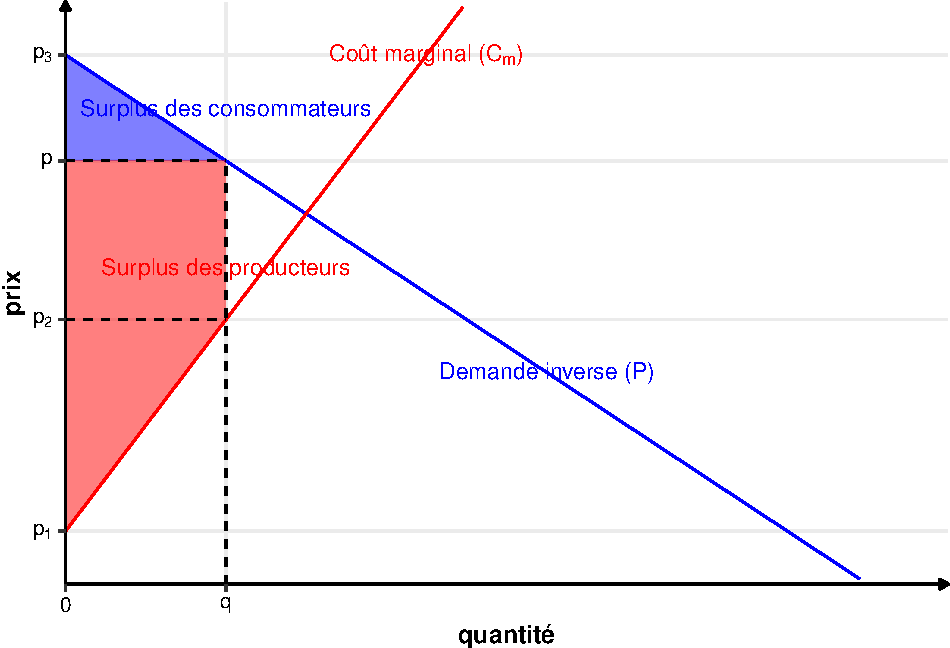
\includegraphics{_main_files/figure-latex/annexesurplus2-1.pdf}
\caption{\label{fig:annexesurplus2}Surplus avec un prix de l'échange \(p\).}
\end{figure}

Le second cas est illustré sur le graphique \ref{fig:annexesurplus3}.
Le prix de l'échange \(p\) est tel que le surplus des consommateurs est un trapèze, et le surplus des producteurs est un triangle.
Dans ce cas, on obtient \(p_2= P(q)\).
Le surplus des consommateurs est donné par :
\[
S_c=\frac{1}{2}\times(p_3-p+p_2-p)\times q
\]
Et le surplus des producteurs par :
\[
S_p=\frac{1}{2}\times(p-p_1)\times q
\]

\begin{figure}
\centering
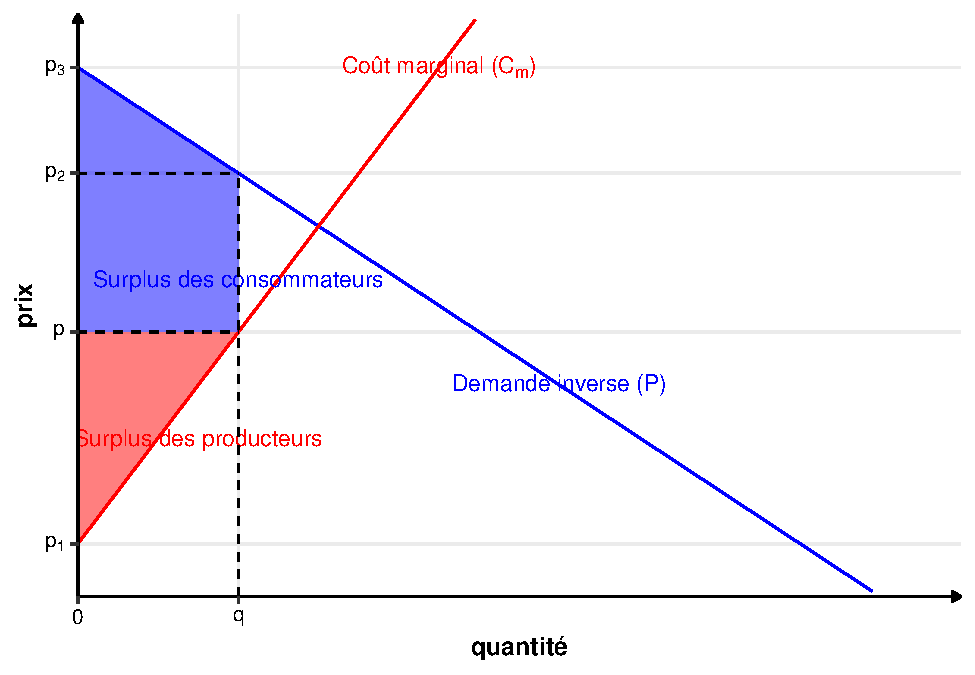
\includegraphics{_main_files/figure-latex/annexesurplus3-1.pdf}
\caption{\label{fig:annexesurplus3}Surplus avec un prix de l'échange \(p\).}
\end{figure}

  \bibliography{book.bib,packages.bib,bibliographie.bib}

\end{document}
